\documentclass[a4paper,11pt]{article}
\pdfoutput=1
\usepackage{jinstpub} % for details on the use of the package,                           please
                     % see the JINST-author-manual
\usepackage{xcolor,soul,framed} %,caption
\usepackage{graphicx}
\usepackage{subcaption}
\usepackage{wrapfig}
\usepackage{mdwmath}
\usepackage{mdwtab}
\usepackage{eqparbox}
\usepackage{url}
\usepackage{dblfloatfix}    % To enable figures at the bottom of page
%\usepackage{kantlipsum}     % for random text
\usepackage{hyperref}
\usepackage[export]{adjustbox}
% \usepackage{longtable}
% \usepackage{booktabs}
% \usepackage{csvsimple}
% longtable support required by pandoc >1.10

%--------------------------------------------------------------------------------%
%%%%%%%%%%%%%%%%%%%%%%%%%%%%%% Document Start %%%%%%%%%%%%%%%%%%%%%%%%%%%%%%%%%%%%
%--------------------------------------------------------------------------------%

\begin{document}
%\bstctlcite{IEEEexample:BSTcontrol}
    \title{Benchmarking Unsupervised Learning Methods in Spectral Imaging}
    
\author[a,1]{Jericho~O'Connell,\note{Corresponding author.}}
\author[a]{Kevin J. Murphy}
\author[a]{Spencer M. Robinson}
\author[b]{Kris~Iniewski}% <-this % stops a space
\author[a]{Magdalena~Bazalova-Carter}

\emailAdd{jerichoo@uvic.ca}

\affiliation[a]{University of Victoria,\\3800 Finnerty Rd, Victoria, BC, Canada}
\affiliation[b]{Redlen Technologies,\\123 - 1763 Sean Heights
Saanichton, BC, Canada}

%--------------------------------------------------------------------------------%
%%%%%%%%%%%%%%%%%%%%%%%%%%%%%% Abstract %%%%%%%%%%%%%%%%%%%%%%%%%%%%%%%%%%%%
%--------------------------------------------------------------------------------%

\abstract{
Data aquired with a 330 $\mu$m pitch  $8\times12$ Cadmium Zinc Telluride detector with five energy bins is utilized to benchmark nine unsupervised clustering algorithms. Each algorithm is benchmarked using single energy (SE), dual energy (DE) and spectral imaging data with clustering results scores based on V-measure. Principle component analysis (PCA), independent component analysis, and non-negative matrix factorization are also benchmarked as dimensional reduction methods for spectral imaging. A phantom with two hard materials (glass, steel) and three soft materials (PVC, polypropylene, and PFTE) all embedded in PMMA was imaged. Analysis used five energy bins for the spectral image, two energy bins for the DE image and a single bin for the SE image. Results show that SE imaging is most capable of hard tissue segmentation using a bayesian gaussian mixture model (BGMM), with a V-measures of 0.84. This was 6.3\% better than DE and 5.0\% better than spectral on this task. Conversely, spectral imaging had the highest V-measure on the soft materials using PCA and a novel interpolating BGMM with a V-measure of 0.71. This was 3.5\% better than DE and 20.3\% better than SE on this task. 

}

\maketitle
% * <jericho.oconnell@icr.ac.uk> 2018-08-29T22:15:14.220Z:
%
% ^.

%--------------------------------------------------------------------------------%
%%%%%%%%%%%%%%%%%%%%%%%%%%%%%% Introduction %%%%%%%%%%%%%%%%%%%%%%%%%%%%%%%%%%%%
%--------------------------------------------------------------------------------%

\section{Introduction}

For the past hundred years, radiography has remained the front line of diagnostic imaging. Due to ubiquity, radiography delivers large amounts of dose to the general population. Compounding this issue, being the first-line of diagnostics, inaccuracies in radiography lead to false-positive findings. These false-positives subject healthy patients to more radiation and increase health care costs. For example, mammography's positive predictive power is as low as 20\% \cite{Skaane2013ProspectiveArbitration., Dickersin2010TheCancer, Kopans1992TheMammography., Mushlin1998EstimatingMeta-analysis, Chiarelli2013DigitalProgram} due to it's high rate of false positives. Further, we see that false-positives are reported to be as high as 60\% for women undergoing screening mammography over 10 years \cite{Kerlikowske2013OutcomesTherapy, Hubbard2011CumulativeMammography}. Thus, we look at new imaging modalities such as spectral and dual energy (DE) as means to improve the false-positive rates in radiography. Or equally provide similar image quality with a lower imaging dose.

% The linear attenuation of X-rays is dependant on the density of the material. The density of the material is independent of the photon energy. If separating a material based on density the energy dependence of the attenuation is therefore not relevant. In contrast, with materials of similar density, the case for many soft tissues, materials cannot be separated based on density. In this case the energy dependence of the attenuation coefficient, characteristic of a material, is used to differentiate materials. This is done through a multi-energy imaging process \cite{Alvarez1976Energy-selectiveTomography.}. Naively one might think the more images at different energies acquired the better the determination of the energy dependence of the attenuation. However, in the original paper on dual energy imaging Alvarez states that two energies is sufficient: With two images we solve for the Compton scattering and photoelectric components in each voxel. These two components fully describe the attenuation in the kV range. Making more than dual energy imaging resultant in dependant information and no gain in tissue differentiation.

Recently, Monte Carlo simulations have shown added benefits in tissue differentiation tasks using spectral CT \cite{Lalonde2016ACT} thus disputing the benefit of multi-energy imaging. Further, in planar imaging, which is the subject of this work, more than two energies has been shown to improve differentiation \cite{OConnell2019OptimalDetector}: Planar images often contain an unknown depth of material, which must also be determined to identify the material. Thus spectral image is hypothesized to aid in planar imaging segmentation tasks. Since spectral and DE imaging are concerned with differentiation of soft materials based on differences in the attenuation rather than the density, new methods are applied to analyze materials. Much of the work in DE CT focused on the calculation of elemental compositions for Monte Carlo dose calculations and thus converts the DE images into the electron density and effective atomic number to characterize the material \cite{Bazalova2008Dual-energyCalculations,Landry2013DerivingCoefficients,Saito2017ABody}. This approach does not work in planar imaging as all pixels in the image must be assumed to be partial volume. This leaves room to explore new methods for segmentation with this modality:

In this work a CZT spectral detector is used with five energy bins. Using five energy bins we have a modality that is in between two better known imaging modalities: On one side we have DE imaging with images at two energies. On the other side hyperspectral imaging with hundreds of images. Hyperspectral imaging is performed at photon energies near the visual spectrum and sees application in very different use cases than DE X-ray imaging. However the data is in the format of a many dimensional energy image and thus has parallels to spectral imaging. In hyperspectral imagining clustering methods have seen success images \cite{Murphy2018UnsupervisedDiffusion,Gillis2012HyperspectralGraphs,Noe2001PartialClustering}. Likewise dimensional reduction is standard in the pre-processing of the images \cite{Mahesh2015HyperspectralMaterials}. With these methods as motivation we apply clustering methods to spectral imagingas well as single and DE imaging.

In SE CT imaging some clustering methods have been applied. Yoa et al. applies a GMM model to segment spinal CT volumes for automated segmentaion in a surgical setting \cite{Yao2004ColonicModels}. Likewise, Li et al. apply a fuzzy c-means segmentation in order to segment colon polyps \cite{Li2008ImprovedRadiography}. However to the best of the authors knowledge there has not been a comprehensive comparison of clustering methods on an X-ray imaging task. This work aims to be the first general comparison of clustering methodologies on a planar imaging task. This work further aims to benchmark performance of single, dual, and spectral clustering methods using data aquired with a Redlen (Redlen Technologies, Saanichton B.C., Canada) CZT spectral detector with five energy bins. Further, a novel interpolating clustering algorithm is proposed for optimal soft tissue segmentation.


%--------------------------------------------------------------------------------%
%%%%%%%%%%%%%%%%%%%%%%%%% Materials/Methods %%%%%%%%%%%%%%%%%%%%%%%%%%%%%%%%%%%%
%--------------------------------------------------------------------------------%

\section{Materials and Methods}
\label{sec:methods}

\begin{figure}[htbp]

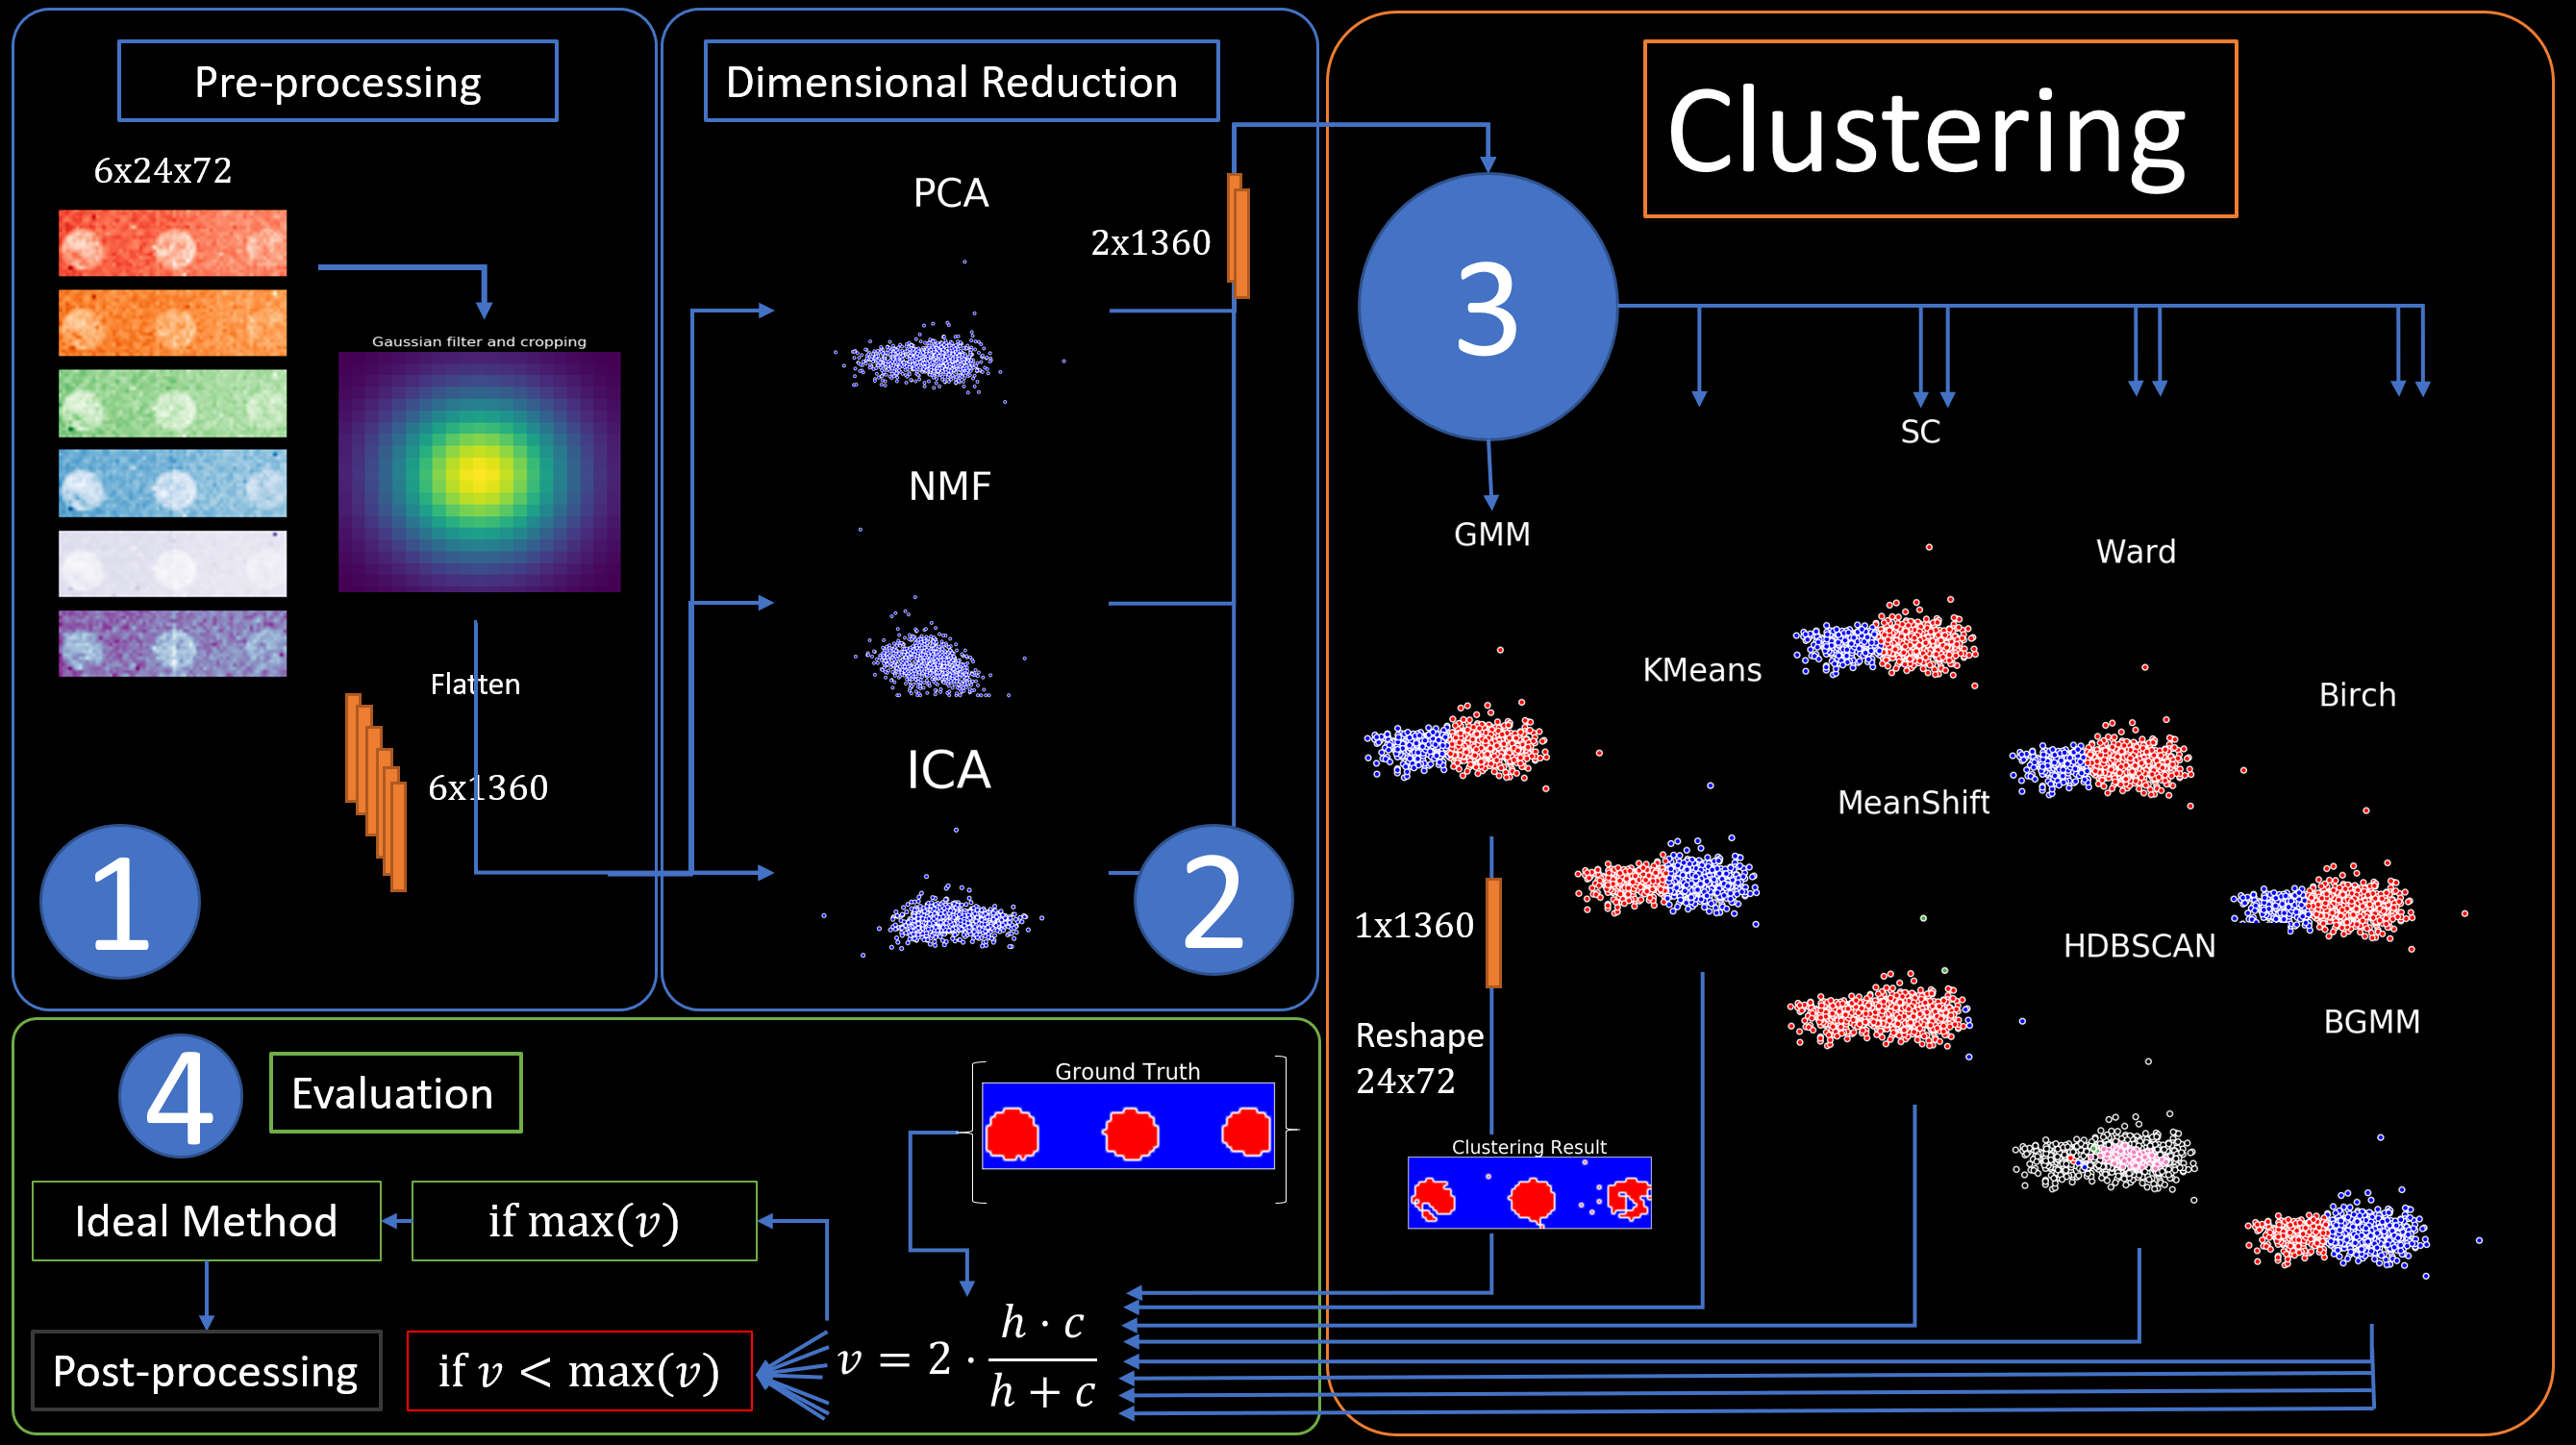
\includegraphics[width=\textwidth]{figures/flow_chart.png}

\caption{A general overview of the workflow is seen, outlining the four general steps of the segmentation method.}
\label{overview}
\end{figure}

\subsection{Data Aquistion}

A full overview of the analysis in this work can be seen in Figure \ref{overview}. Data was acquired as follows:

X-ray scans were performed on a PMMA phantom with five materials (steel, glass, PVC, polypropylene, and PTFE). PVC, polypropylene and PTFE were considered to be the soft materials while glass and steel were considered the hard materials. These materials were used as a benchmark as they are freely available and cover a range of density similar to the range seen in human tissues.

Data was acquired using a CZT detector with a 8$\times$12 mm imaging array from Redlen Technologies. The 330 $\mu$m pitch high-flux CZT detector is 2mm thick and is able to operate at 250 $\frac{Mcps}{mm^2}$ without any signs of polarization. Travel Heat Method (THM) was adopted by Redlen Technologies when growing the CZT crystals used in the detector. These crystals were placed in a sensor that is connected to a photon counting ASIC which operates at rates of up to 62.5 $\frac{Mcps}{channel}$. This ASIC communicates with an external PC though LVDS I/Os via a programmable FPGA. The energies of photons incident with the detector are sorted into five energy bins by the ASIC. In the case of this experiment the energy bins were set to 16-33 keV, 33-41 keV, 41-50 keV, 50-90 keV, and 90-120 keV.

The detector and X-ray source were both mounted on vertical and horizontal linear motion stages from Newport Corporations. These stages were oriented perpendicular to each other to allow for easy navigation while imaging the phantom, which was mounted between these two stages. The X-ray source used was a module XRS-160 from Comet Technologies. An image of the experimental setup can be seen in Figure \ref{figure:setup} a). 

The PMMA phantom block as imaged in Figure \ref{figure:setup} c) was placed on the stage and the 3 smallest inserts of each material were imaged. To image these materials each at different heights, the CZT detector and X-ray source were moved vertically in a uniform manner allowing for each material to be centered without any motion of the phantom block itself. Air scans were completed for each data acquisition and could then be processed using MATLAB (The Mathworks, Natick, MA) for image reconstruction and CNR calculations for each contaminate. During all scans the X-ray tube was using a cone beam operating at 1mA, 120 kV, with a 1mm focal spot. A DE image was created for each spectral image by summing over the first two and last three bins of the image while a SE image was created by summing over all of the bins.


\begin{wrapfigure}{R}{0.5\textwidth}
  
  \begin{center}
    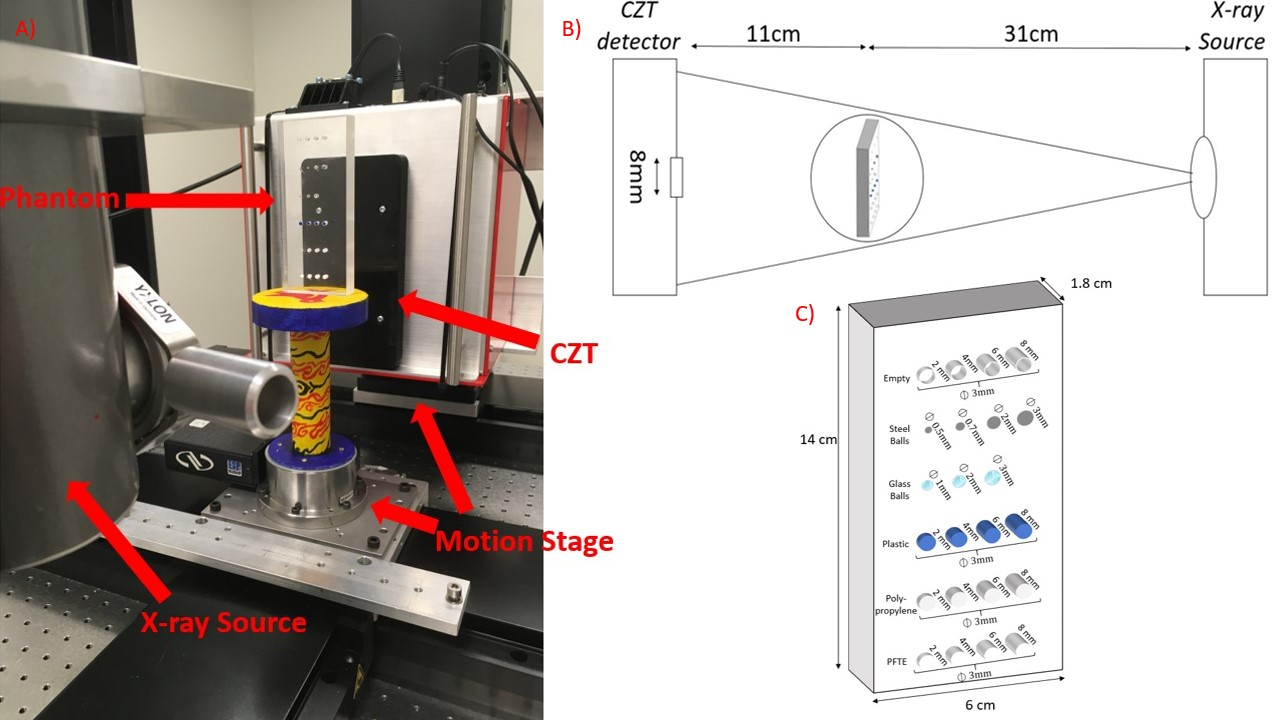
\includegraphics[width=0.48\textwidth]{FullFigure.jpg}
  \end{center}
  
  \caption{a) Shows an image of the lab after data was acquired with different components as labeled. b) Is a schematic of the lab with distances from source to detector labeled. c) The layout for the phantom used with sizes of contaminates as labeled.}
  \label{figure:setup}
\end{wrapfigure}

\subsection{Image Segmentation}
\subsubsection{Overview}

Image segmentation was undertaken as a multistage process. Here we borrow from hyperspectral imaging; Mahesh et al. \cite{Mahesh2015HyperspectralMaterials} state that the main steps in hyperspectral images segmentation include pre-processing of data, dimensional reduction, enhancement of spectral responses, and component detection or classification. Using this as a framework for spectral imaging, similar methods are applied. These steps can also be seen in Figure \ref{overview}. An exception being the enhancement of spectral response is not a step at this time, as the modelling of the spectral response of the CZT detector is beyond the scope of this study.

\subsubsection{Pre-processing of Data}

After data aquisition, data pre-processing was performed using MATLAB 2017b (The MathWorks, Natick, USA). The images were first cropped to remove the non-uniform edge pixels in some parts of the detector. Dead pixels were found manually and replaced with NaN values in the image. These NaN values were then interpolated to be the average of the surrounding eight pixels. The images were then smoothed using a two dimensional gaussian filter with a standard deviation of 0.5 to reduce the noise in the image. The six input images after the initial pre-processing are shown in Figure \ref{demonstrating_bins}.

\begin{figure}[htbp]

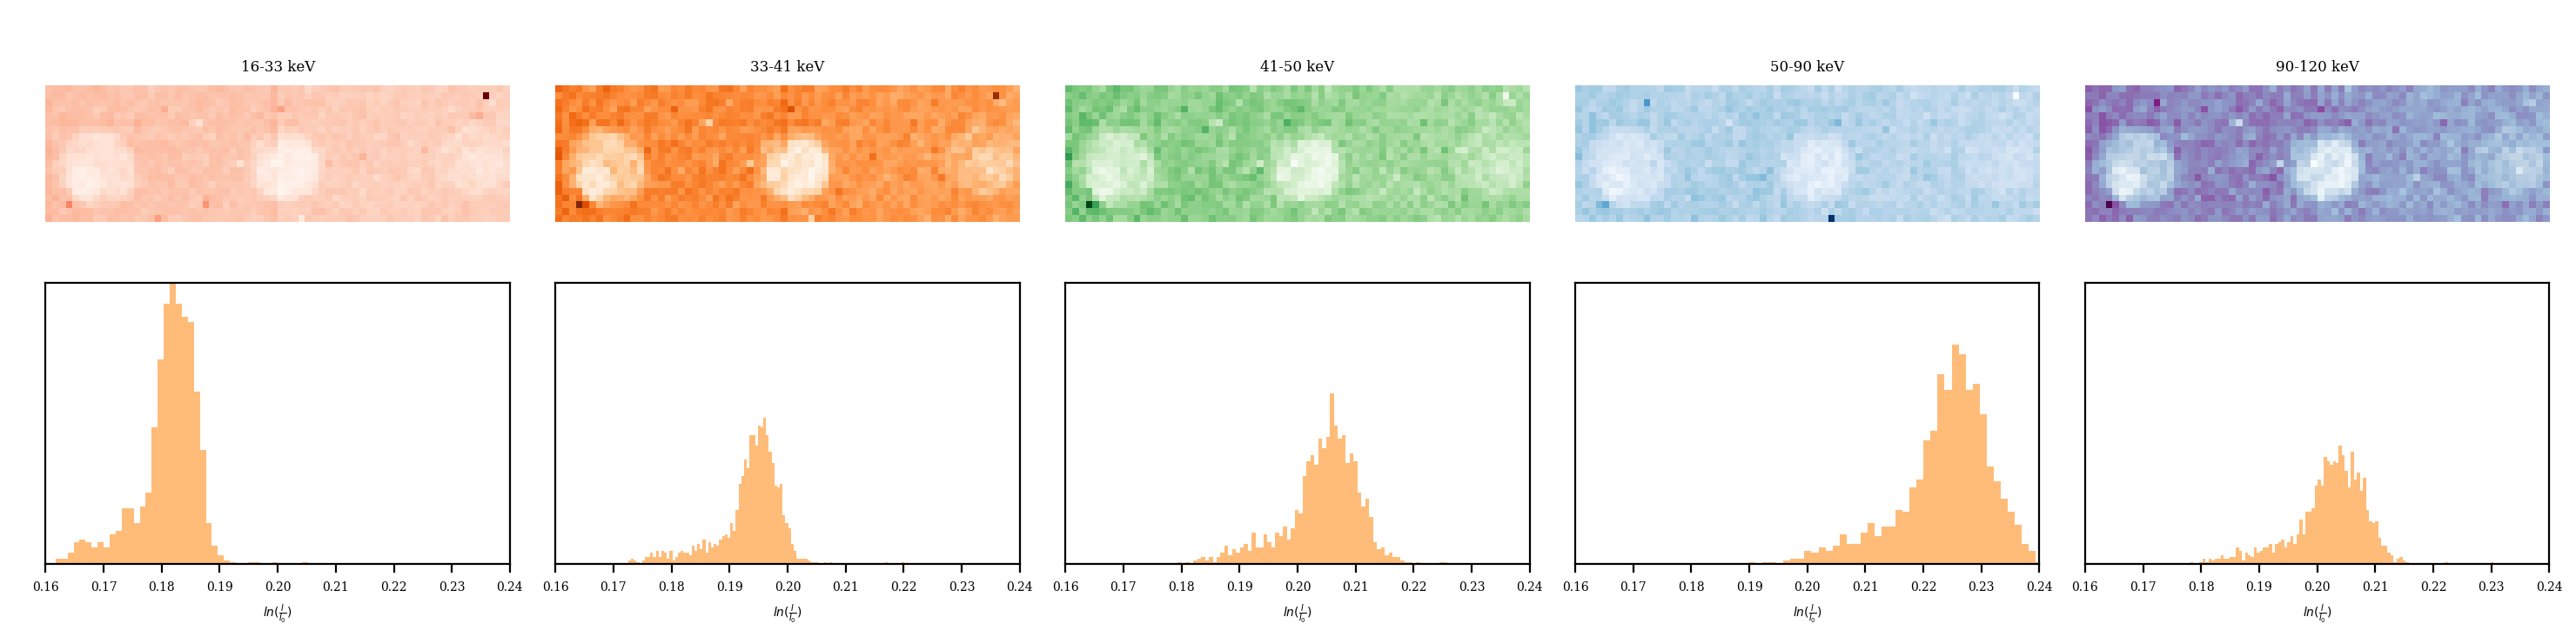
\includegraphics[width=\textwidth]{figures/poly_figure2.png}

\caption{The six energy bins for the image of PMMA embedded with poly-propylene are shown with different colormaps corresponding to their energy, red being lower energy while violet is higher energy. A histogram of the log intensity corresponding to each image is shown below the respective image.}
\label{demonstrating_bins}
\end{figure}

\subsubsection{Dimensional Reduction}

\begin{wrapfigure}{R}{0.5\textwidth}
  
  \begin{center}
    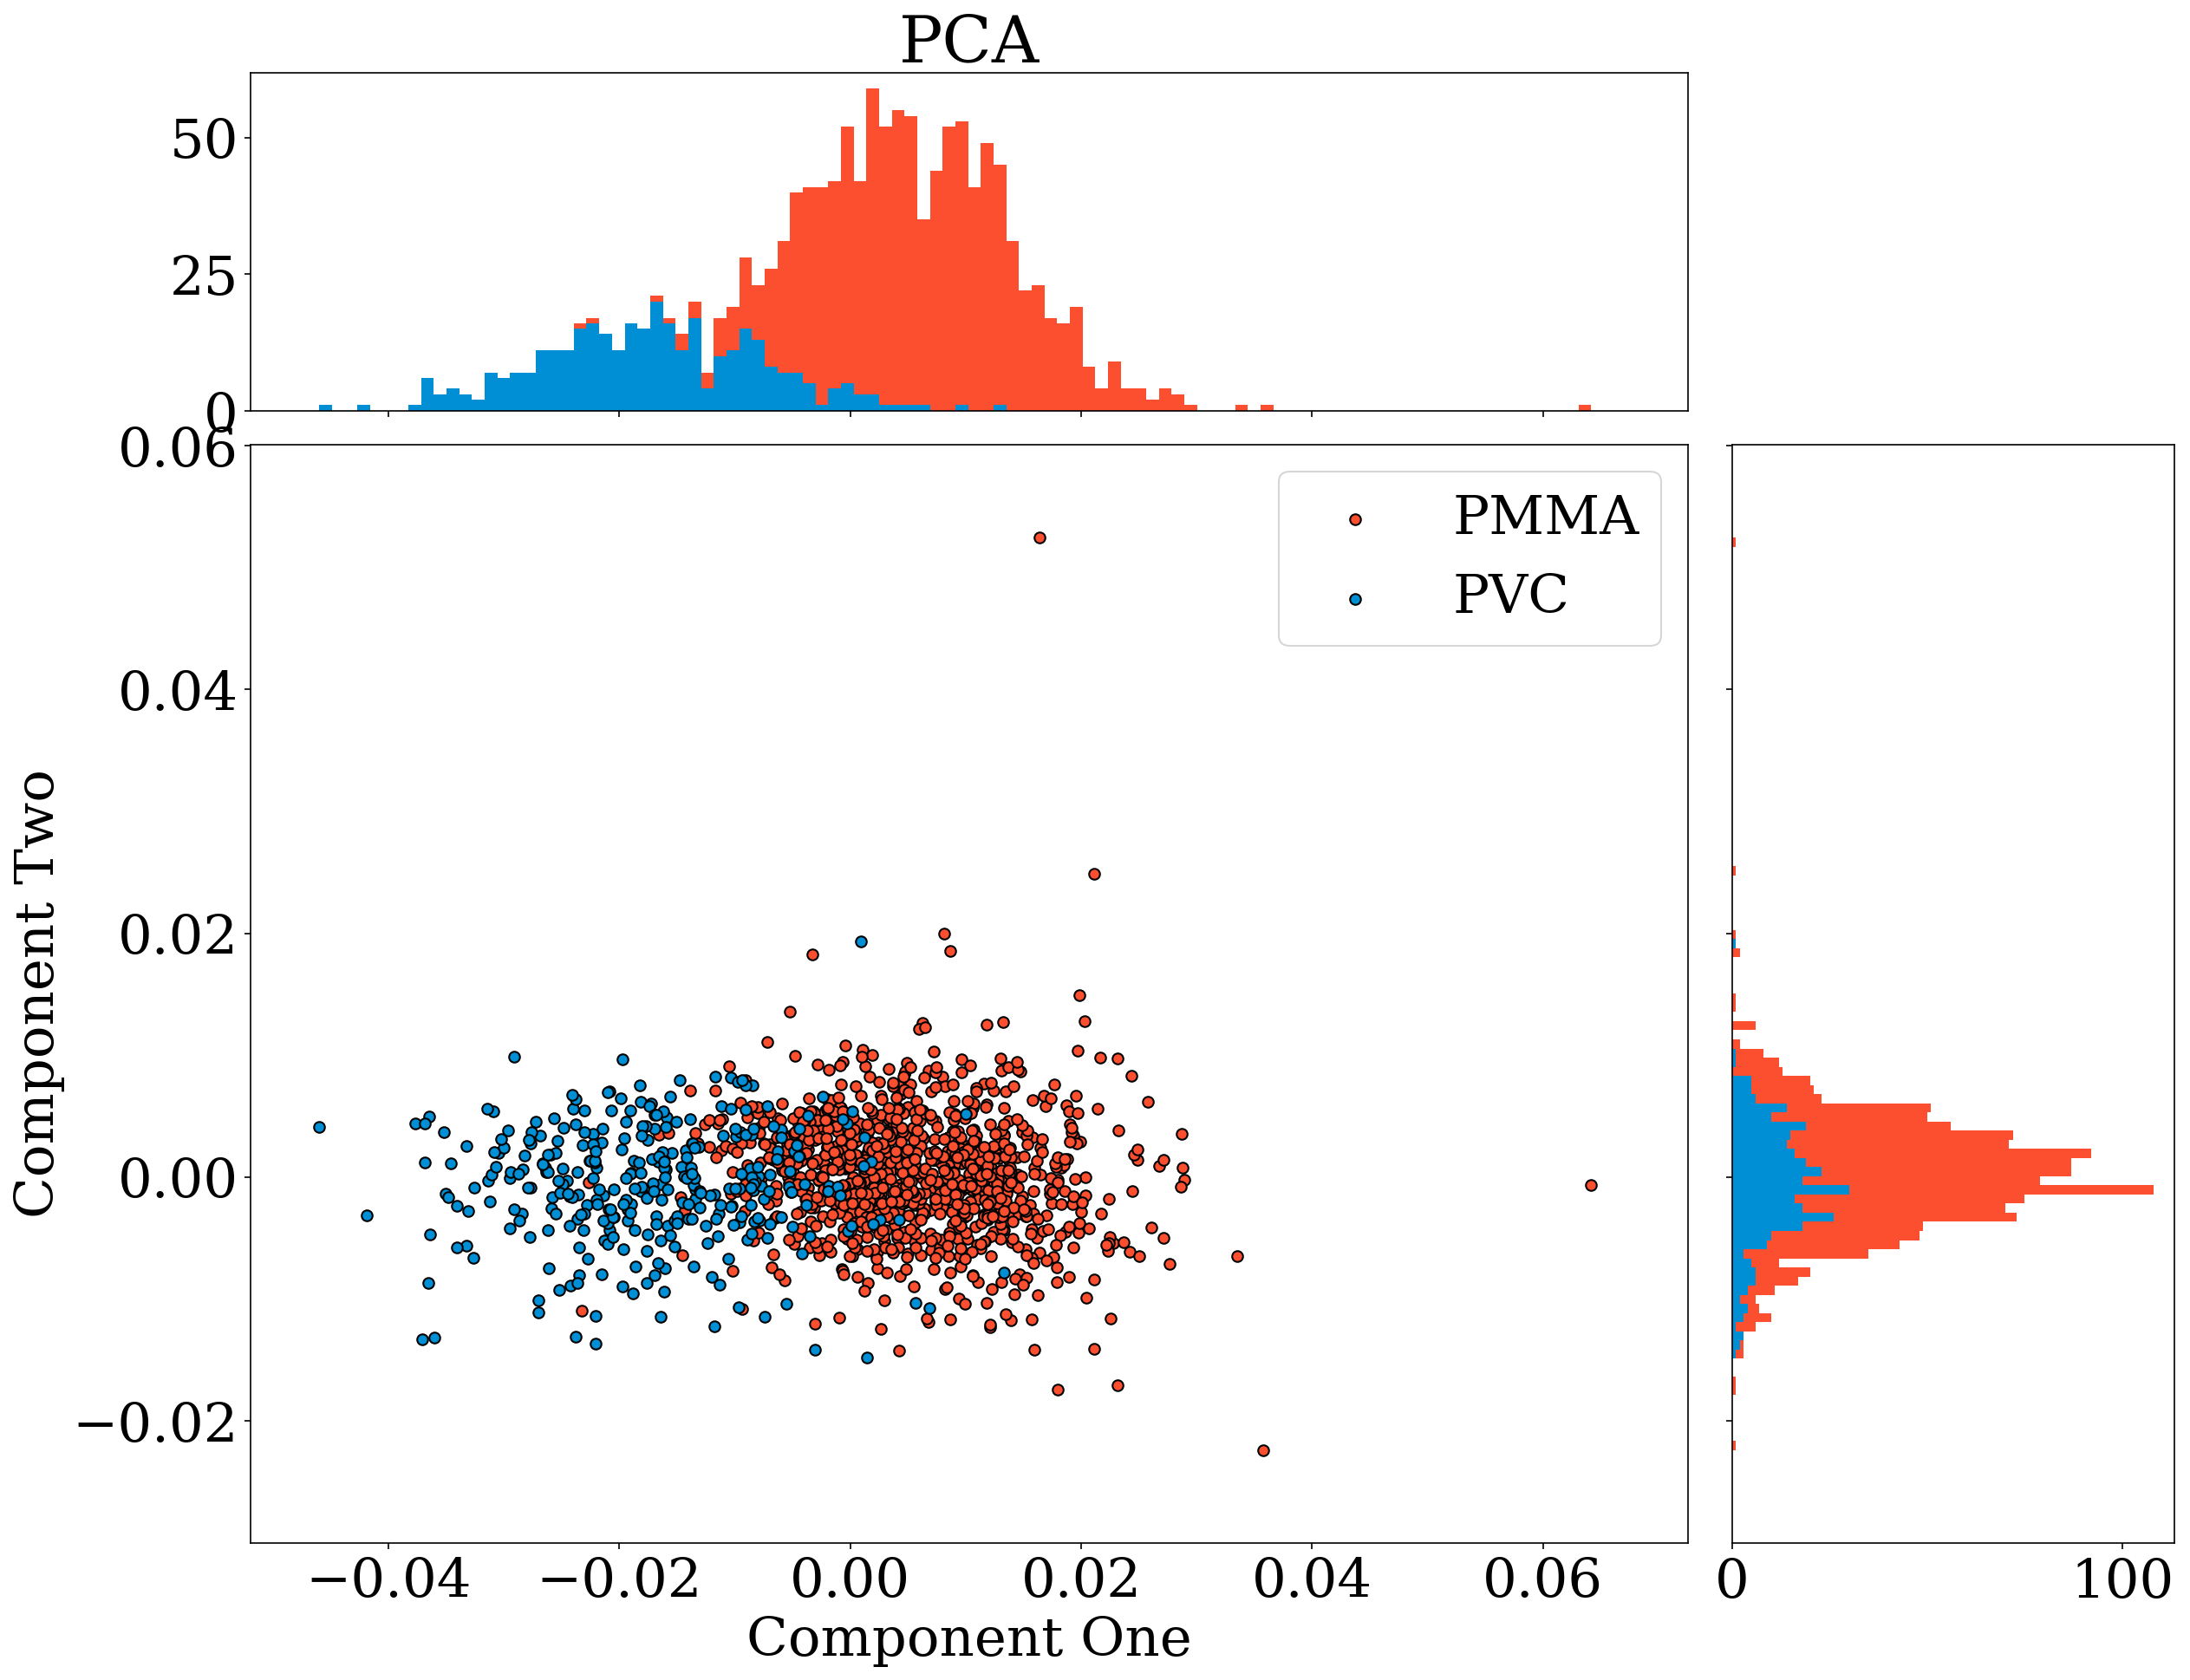
\includegraphics[width=0.48\textwidth]{figures/PCAnone.png}
  \end{center}
  
  \caption{The first two principle components of the PTFE image displayed as a scatter plot.}
  \label{PCA}
  
\end{wrapfigure}

Dimensional reduction methods were applied in this work to increase class separation and reduce noise in the data, methods were implemented in Python (Python Software Foundation) using sci-kit learn \cite{Pedregosa2011Scikit-learn:Python}. The three dimensional reduction thought suitable for this task were principle component analysis (PCA), independent component analysis (ICA), and non-negative matrix factorization (NMF). A visualization of the effect of reducing the data to two dimensions can be seen in Figures \ref{PCA}, \ref{ICA}, and \ref{NMF}.

\subsubsection{Principal Component Analysis}

The first data reduction method employed in this study was Principle Component Analysis (PCA). PCA decomposes the covariance matrix of the feature space into eigenvalues and eigenvectors. Sorting the eigenvectors in terms of the magnitude of their eigenvalue to find the directions of highest variance in the data. The data is then projected into a lower dimensional space defined by the eigenvectors with the largest eigenvalues. This space is by definition orthogonal. This method results in a loss of information, however this loss of information is usually relatively small and ideally the discarded dimensions in the data amount to noise. PCA can be seen in Figure \ref{PCA}. PCA is fast, linear and sees application in many domains. Jolliffe et al. \cite{Jolliffe2016PrincipalDevelopments.} present a more in depth overview of PCA and it's recent applications.

% \begin{wrapfigure}{R}{0.33\textwidth}
  
%   \begin{center}
%     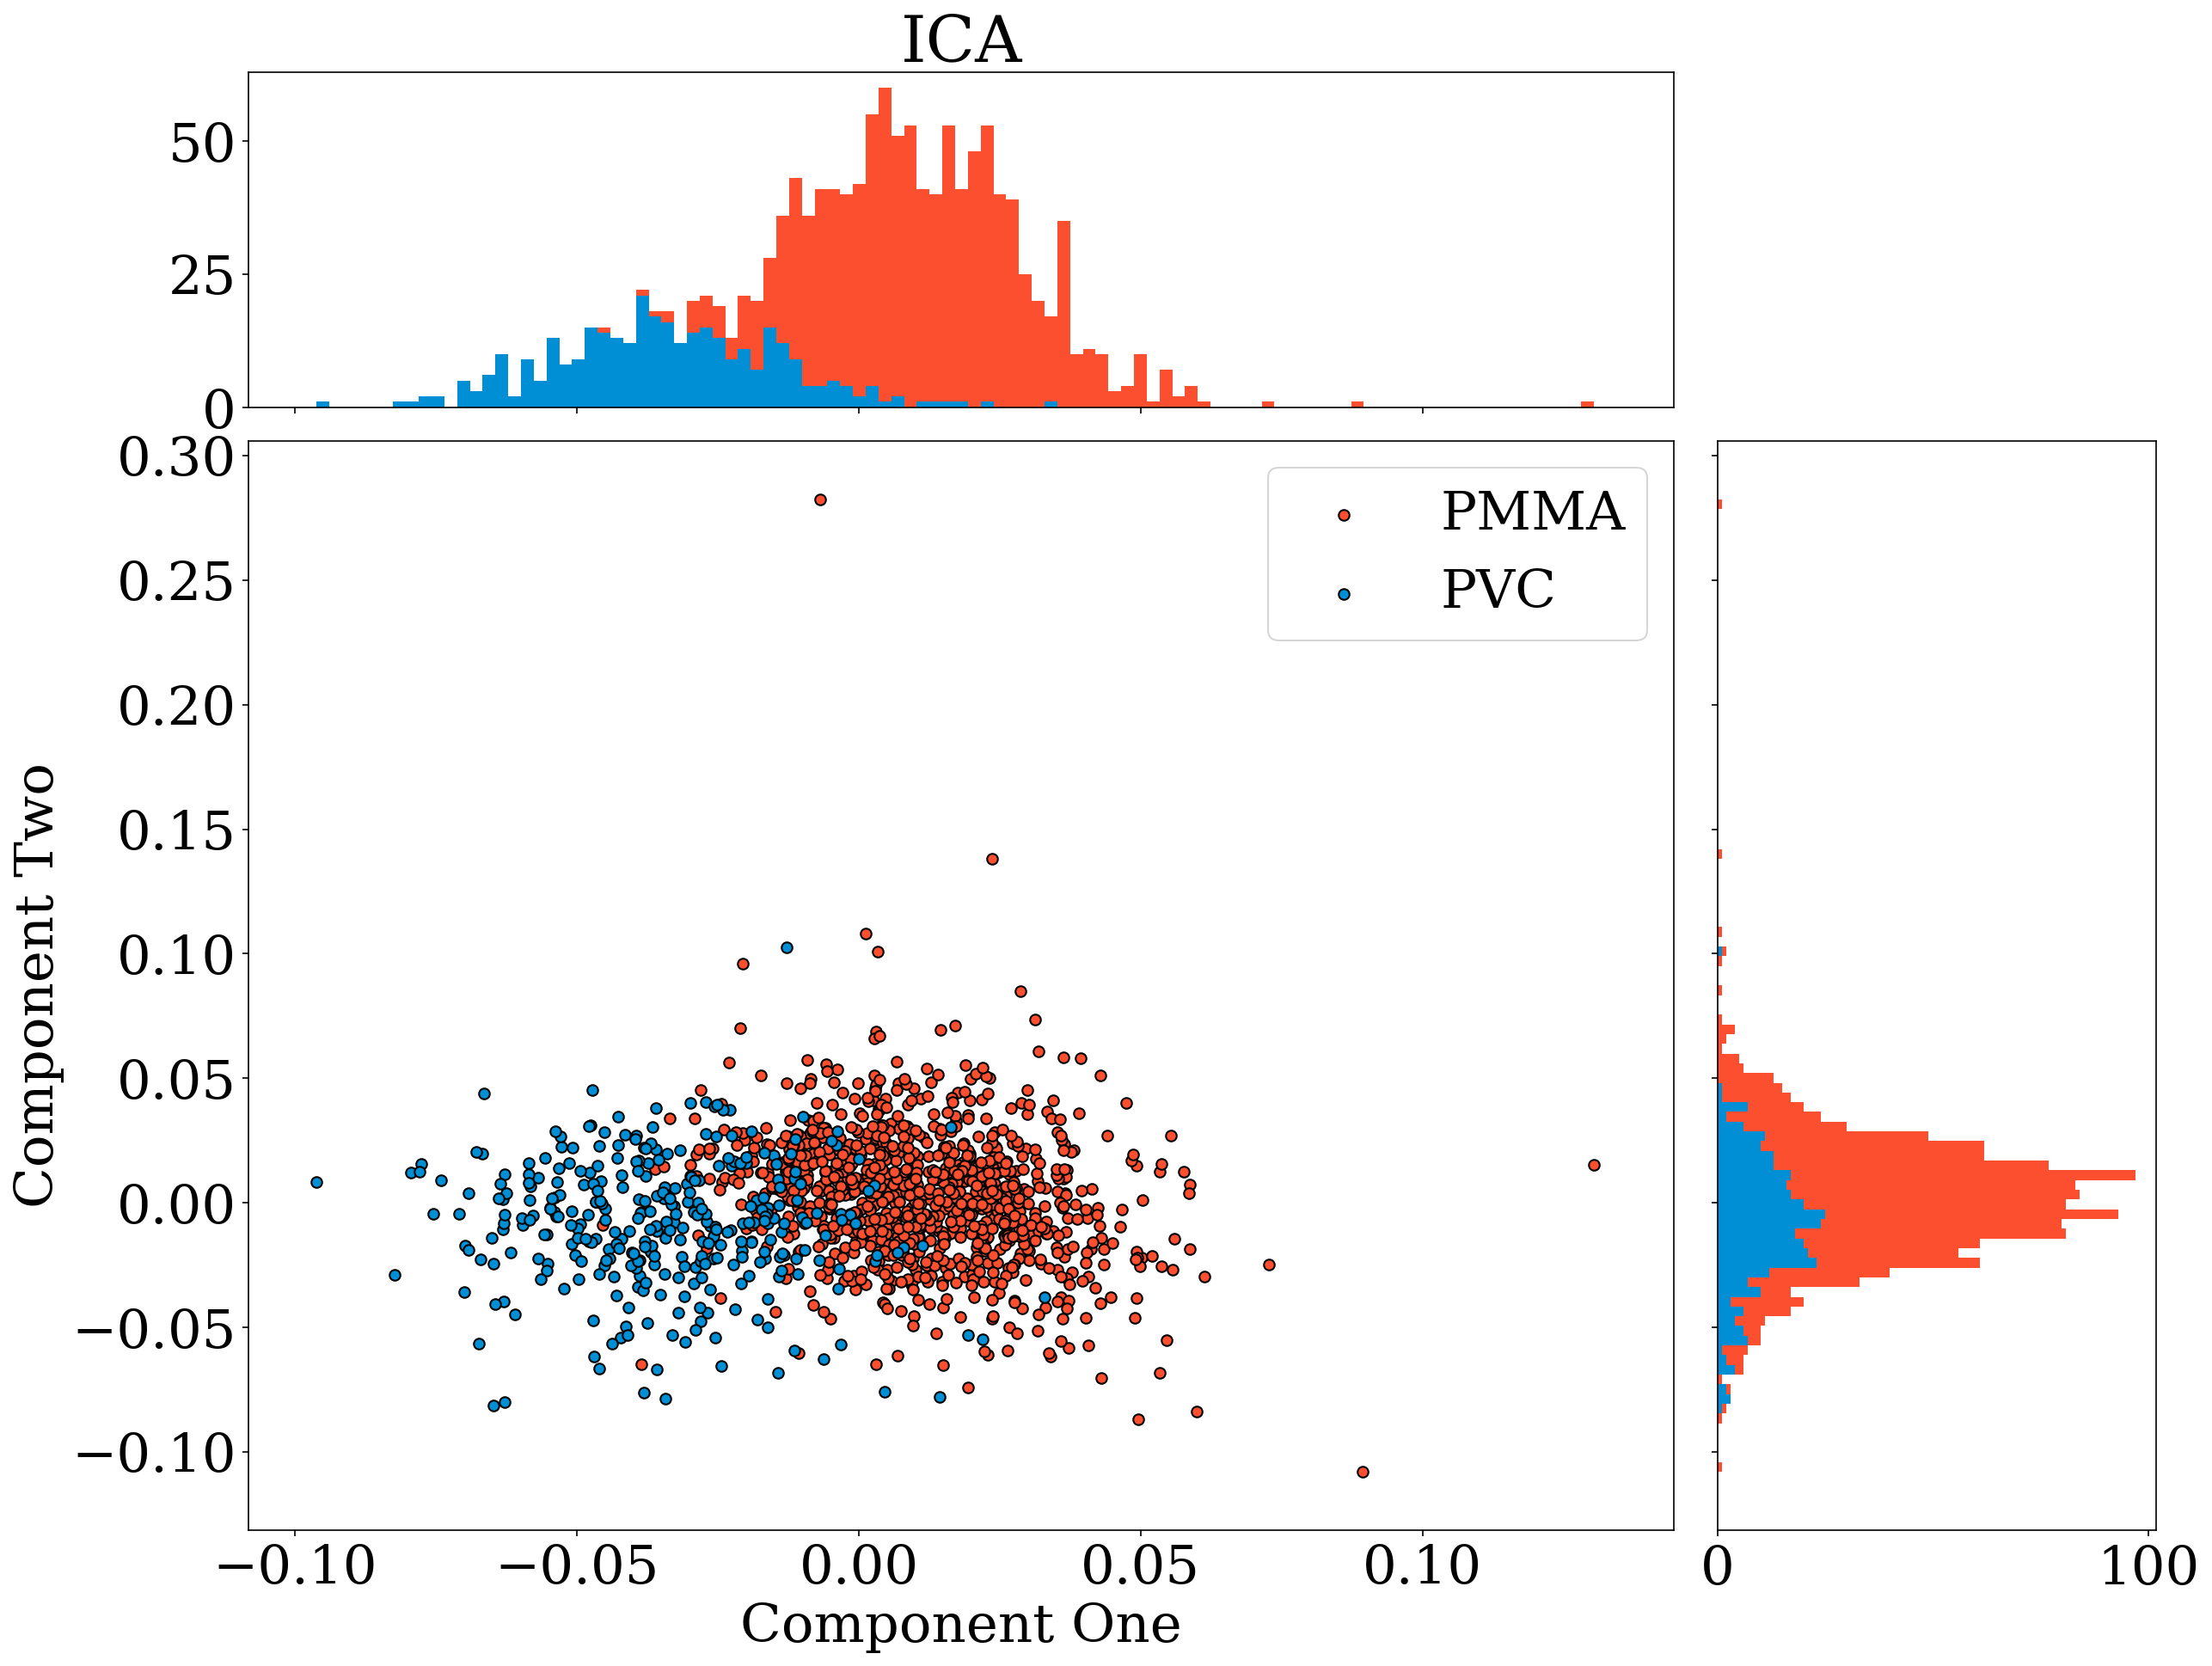
\includegraphics[width=0.33\textwidth]{figures/ICAnone.png}
%   \end{center}
  
%   \caption{The first two independent components of the data displayed as a scatter plot.}
  
%   \label{ICA}
% \end{wrapfigure}

\subsubsection{Independent Component Analysis}

Used for blind source seperation in time series analysis, independant component analysis (ICA) separates a mixed signal into its constituent signals. ICA is also used in hyperspectral imaging \cite{Villa2009OnAnalysis}. Using ICA we frame the segmentation of the two images as a decomposition problem in which the image is a weighted addition of two signals. Idealy these signals would be the background material (PMMA) and the material of interest (eg. PTFE). A demonstration of using ICA on PTFE embedded in PMMA can be seen in Figure \ref{ICA}. A more in depth explanation of ICA can be found in appendix. The algorithm used for ICA in this work was the FastICA \cite{Hyvarinen2000IndependentApplications} algorithm implemented in sci-kit learn.

\begin{wrapfigure}{R}{0.5\textwidth}
  \begin{center}
    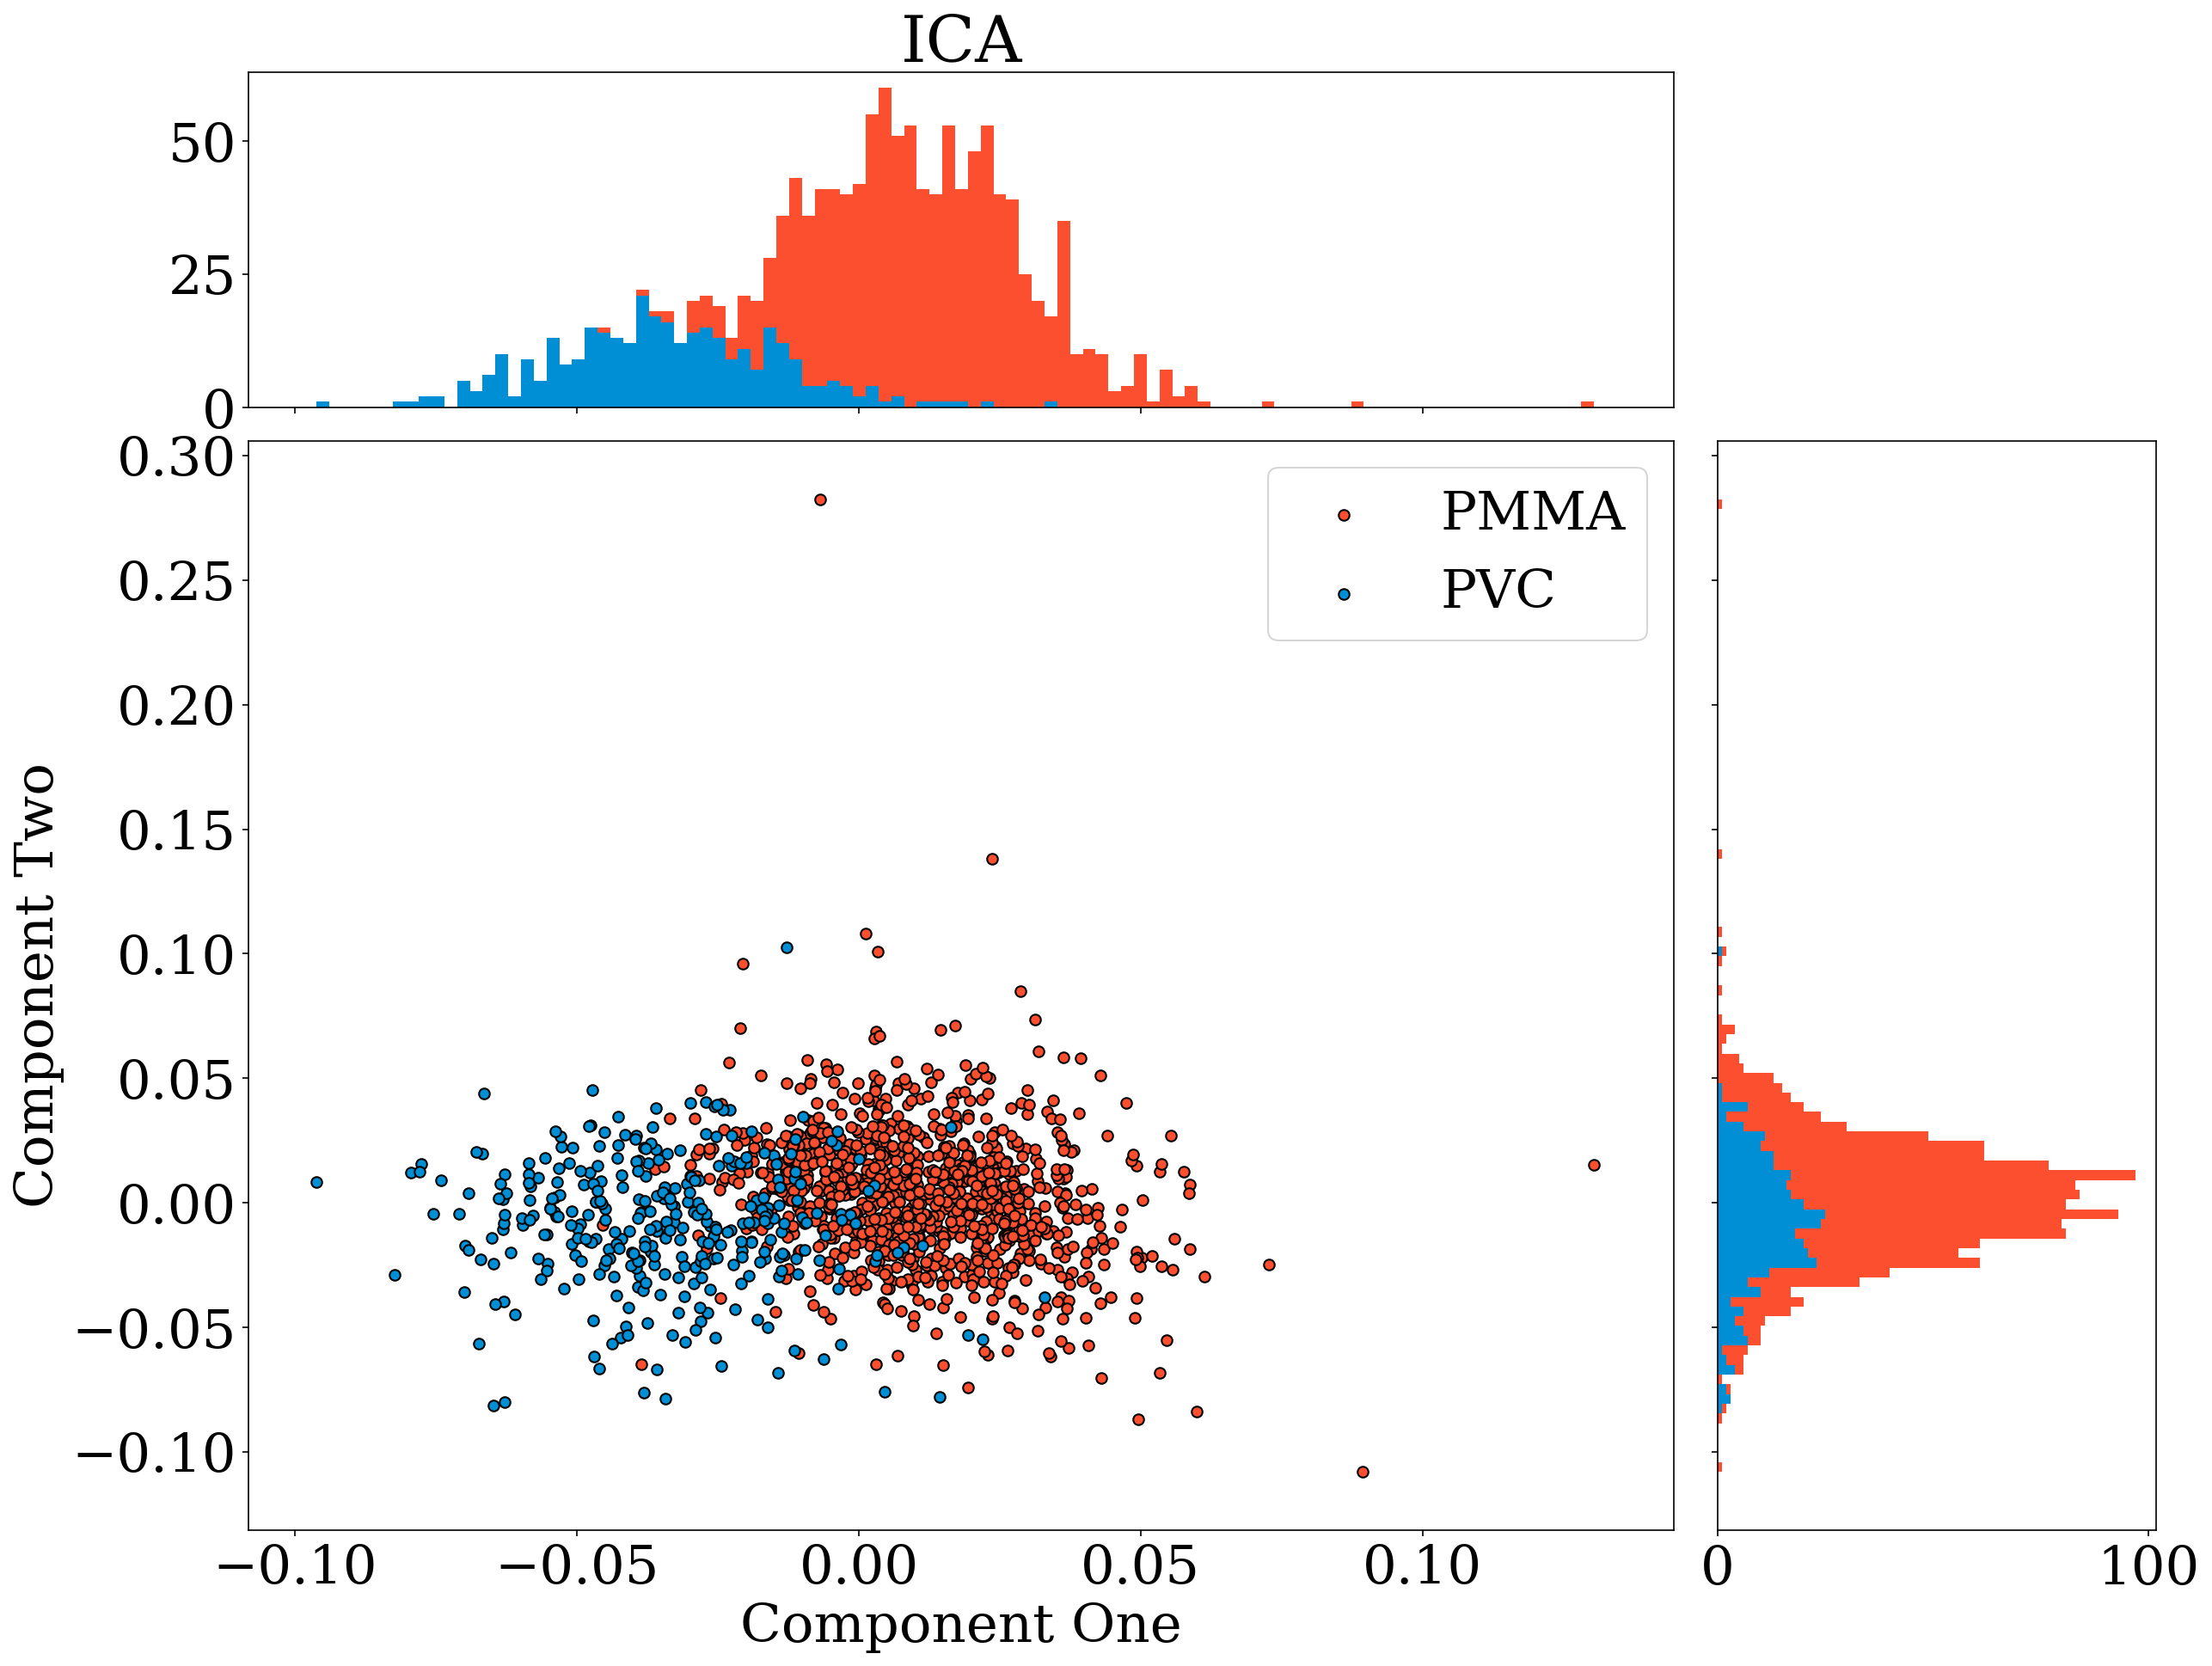
\includegraphics[width=0.48\textwidth]{figures/ICAnone.png}
  \end{center}
  
  \caption{The first two independent components of the PTFE image displayed as a scatter plot.}
  
  \label{ICA}  
  \begin{center}
    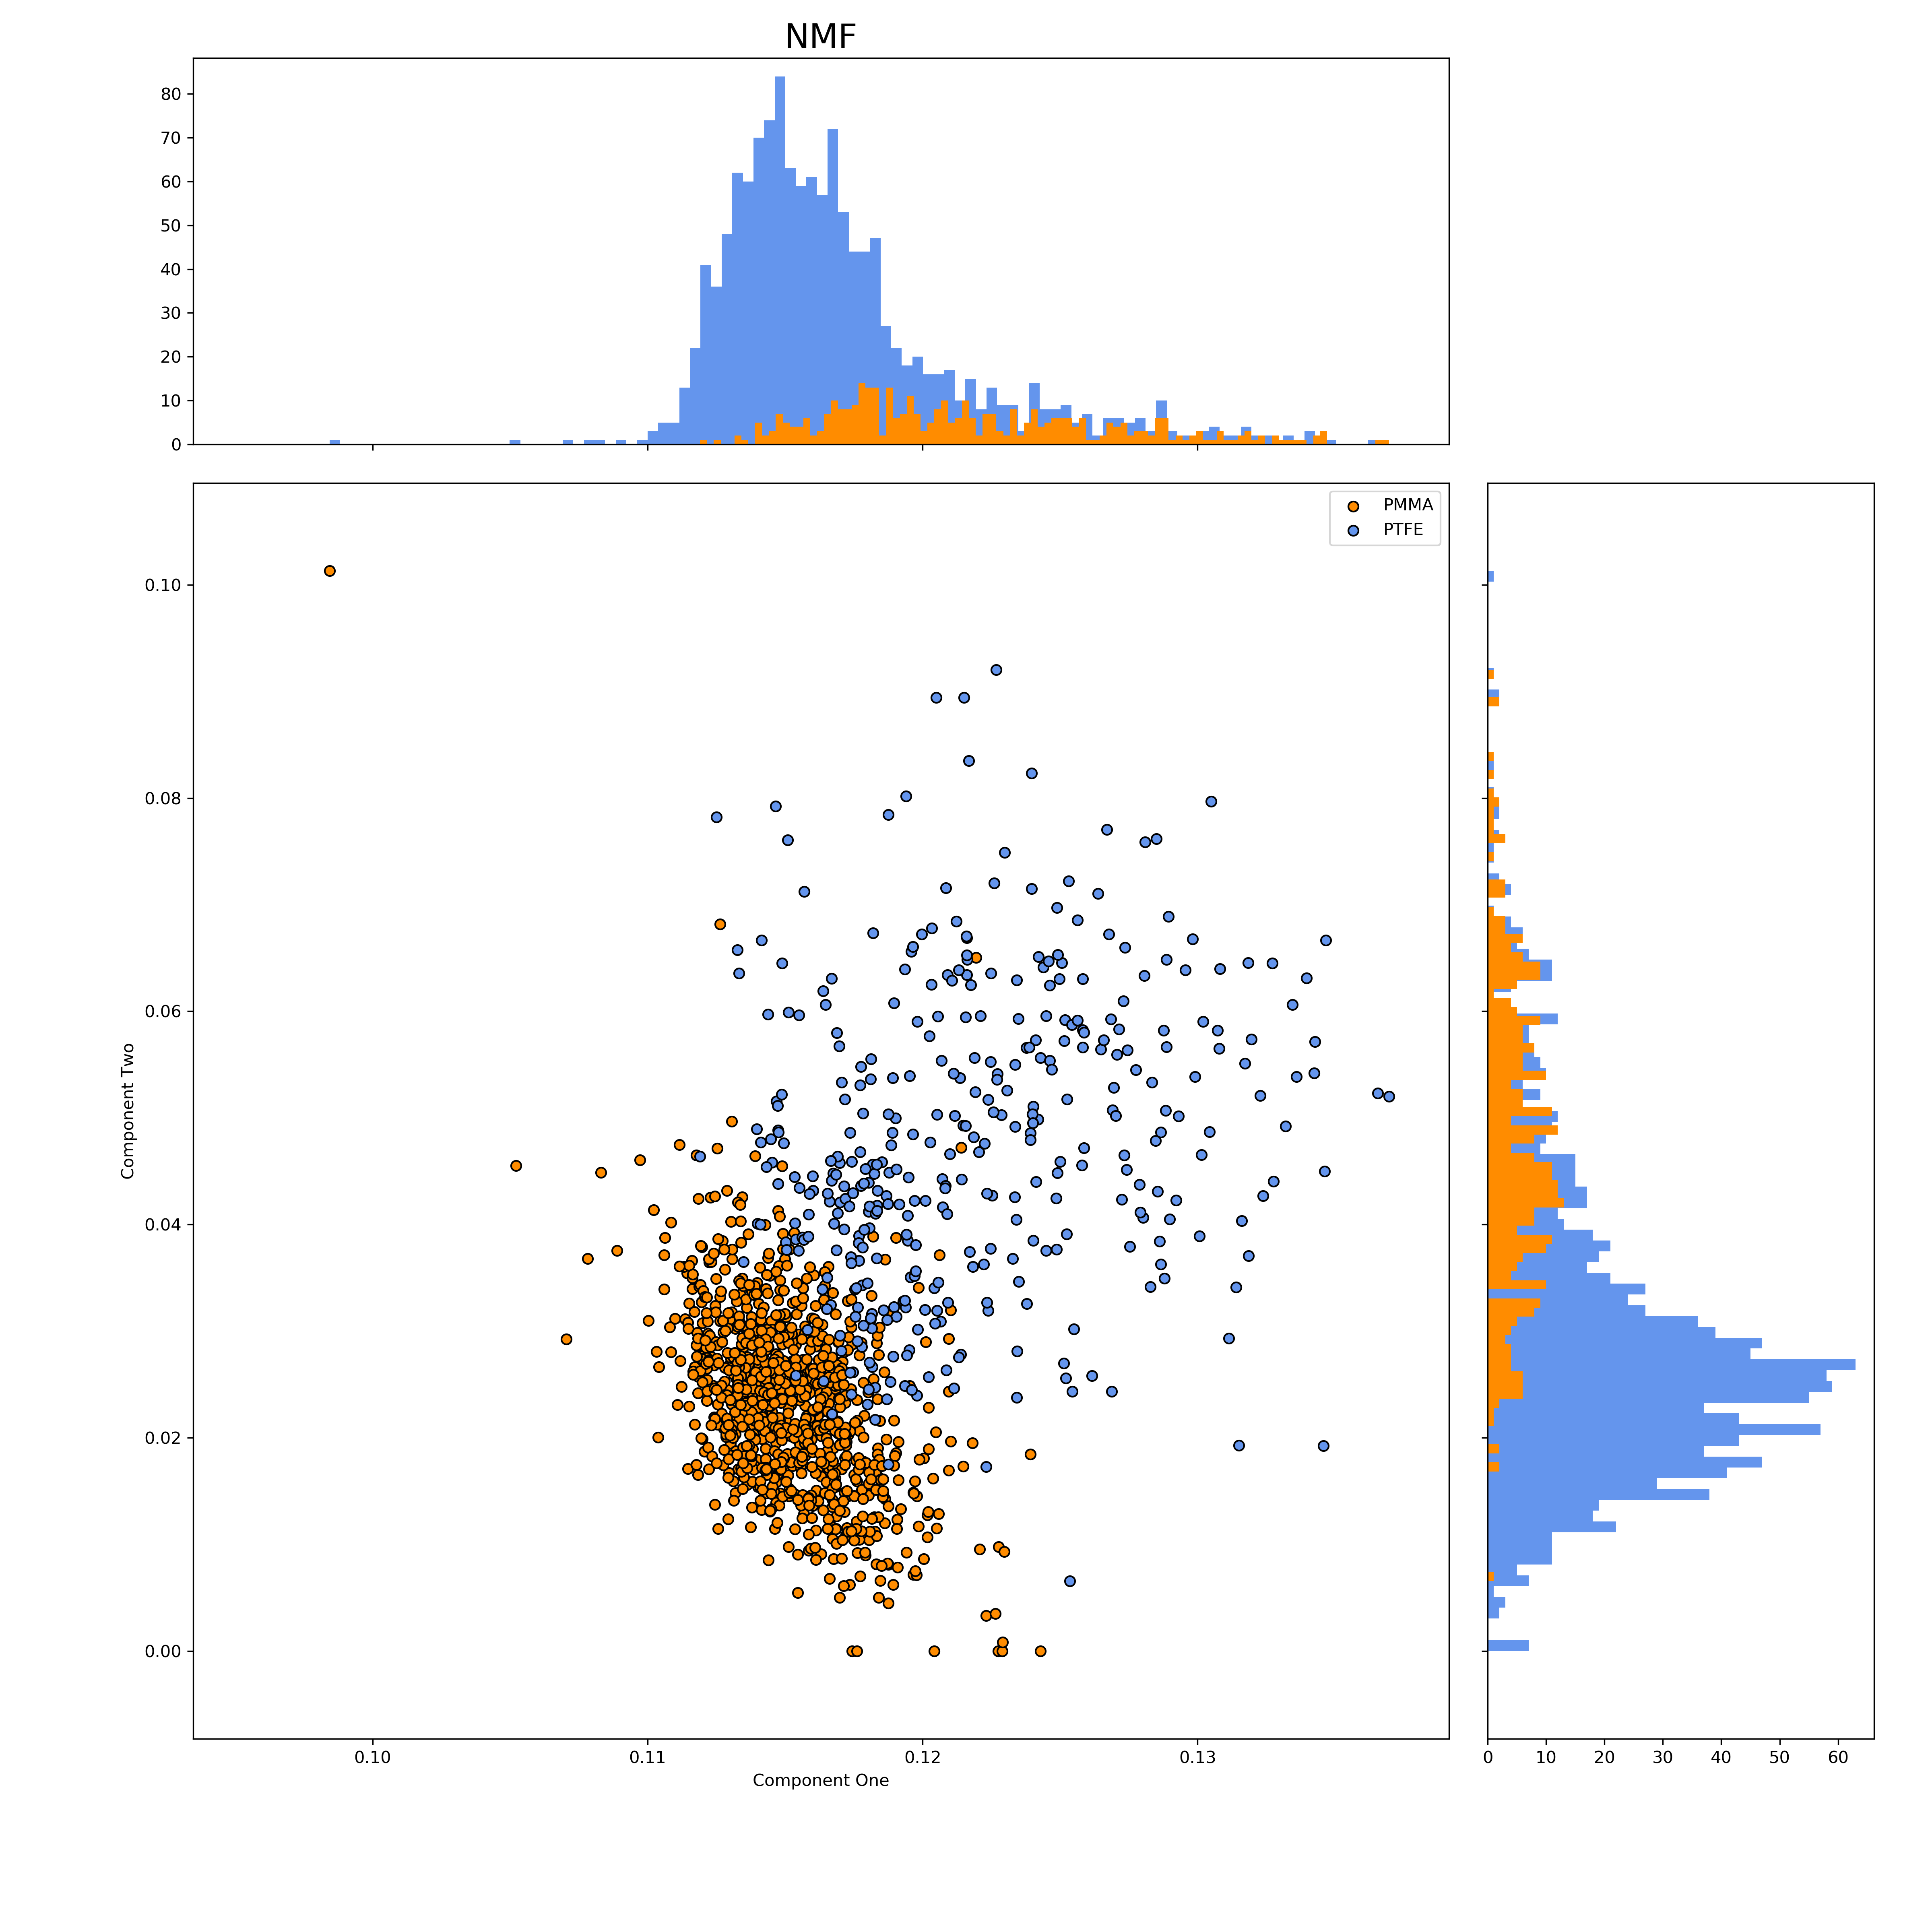
\includegraphics[width=0.48\textwidth]{figures/NMFnone.png}
  \end{center}
  
  \caption{The first two non-negative factorization components of the PTFE image displayed as a scatter plot.}
  
  \label{NMF}
\end{wrapfigure}

\subsubsection{Non-negative Matrix Factorization}

NMF assumes the Matrix $V$ is the product of the two matrices $W$ and $H$ such that : $V = WH$. 

When multiplying matrices the dimension of the factor matrices $W$ and $H$ may be much less that the product matrix. One can think of the two factor matrices as a feature matrix $W$ and a coefficient matrix $H$.

Thus, if one can find matrices $W$ and $H$ that have fewer dimensions than $V$, one can reconstruct the matrix $V$ in the lower dimensional space defined by $W$. To find the matrices $W$ and $H$ numerically we try to minimize the error defined by:

\begin{equation}
\min_{W,H} || V - WH ||, ( W \geq 0, H \geq 0 )
\end{equation}

This was done in using scikit-learn's NMF function, minimizing using the gradient descent algorithm. A demonstration of NMF on PTFE embedded in PMMA can be seen in Figure \ref{NMF}.

\subsection{Clustering Methods}

\subsubsection{K-means}

The first clustering method implemented was K-means clustering. K-means was implemented using the k-means++ algorithm \cite{ArthurK-means++:Seeding}. Different distance metrics were used, however none of the distance metrics tested improved performance over the squared euclidean distance, thus squared euclidean distance was used. K-means is a general purpose, fast and scalable clustering algorithm. Like many of the methods examined K-means requires the parameter $K$ which describes the number of clusters in the data. This parameter can be hard to estimate in some cases. Methods for defining the parameter $K$ will be seen in the following metrics section.

\begin{figure}[t!]
    \centering
    \begin{subfigure}[b]{0.48\textwidth}
        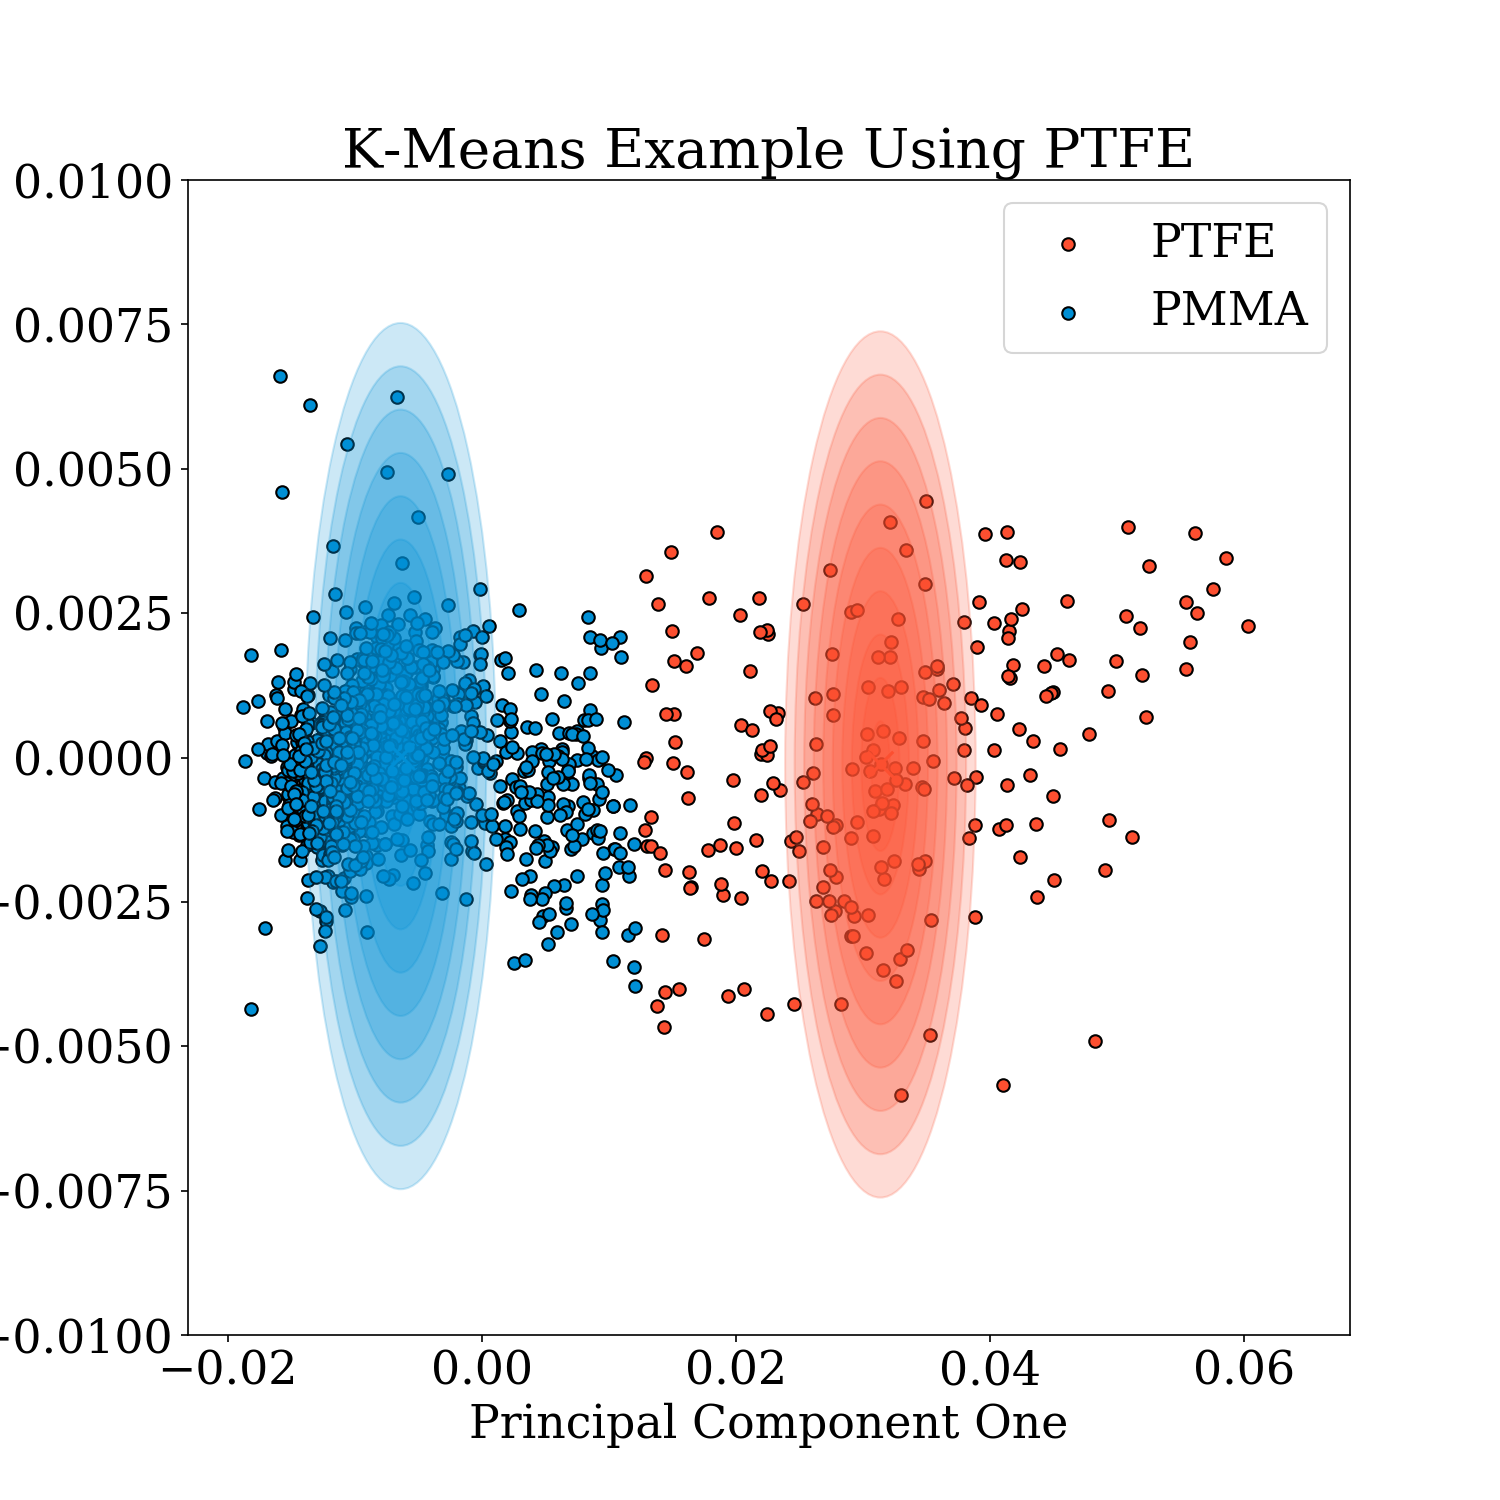
\includegraphics[width=\textwidth]{figures/Kmeans.png}
    \end{subfigure}
    ~ %add desired spacing between images, e. g. ~, \quad, \qquad, \hfill etc. 
      %(or a blank line to force the subfigure onto a new line)
    \begin{subfigure}[b]{0.48\textwidth}
        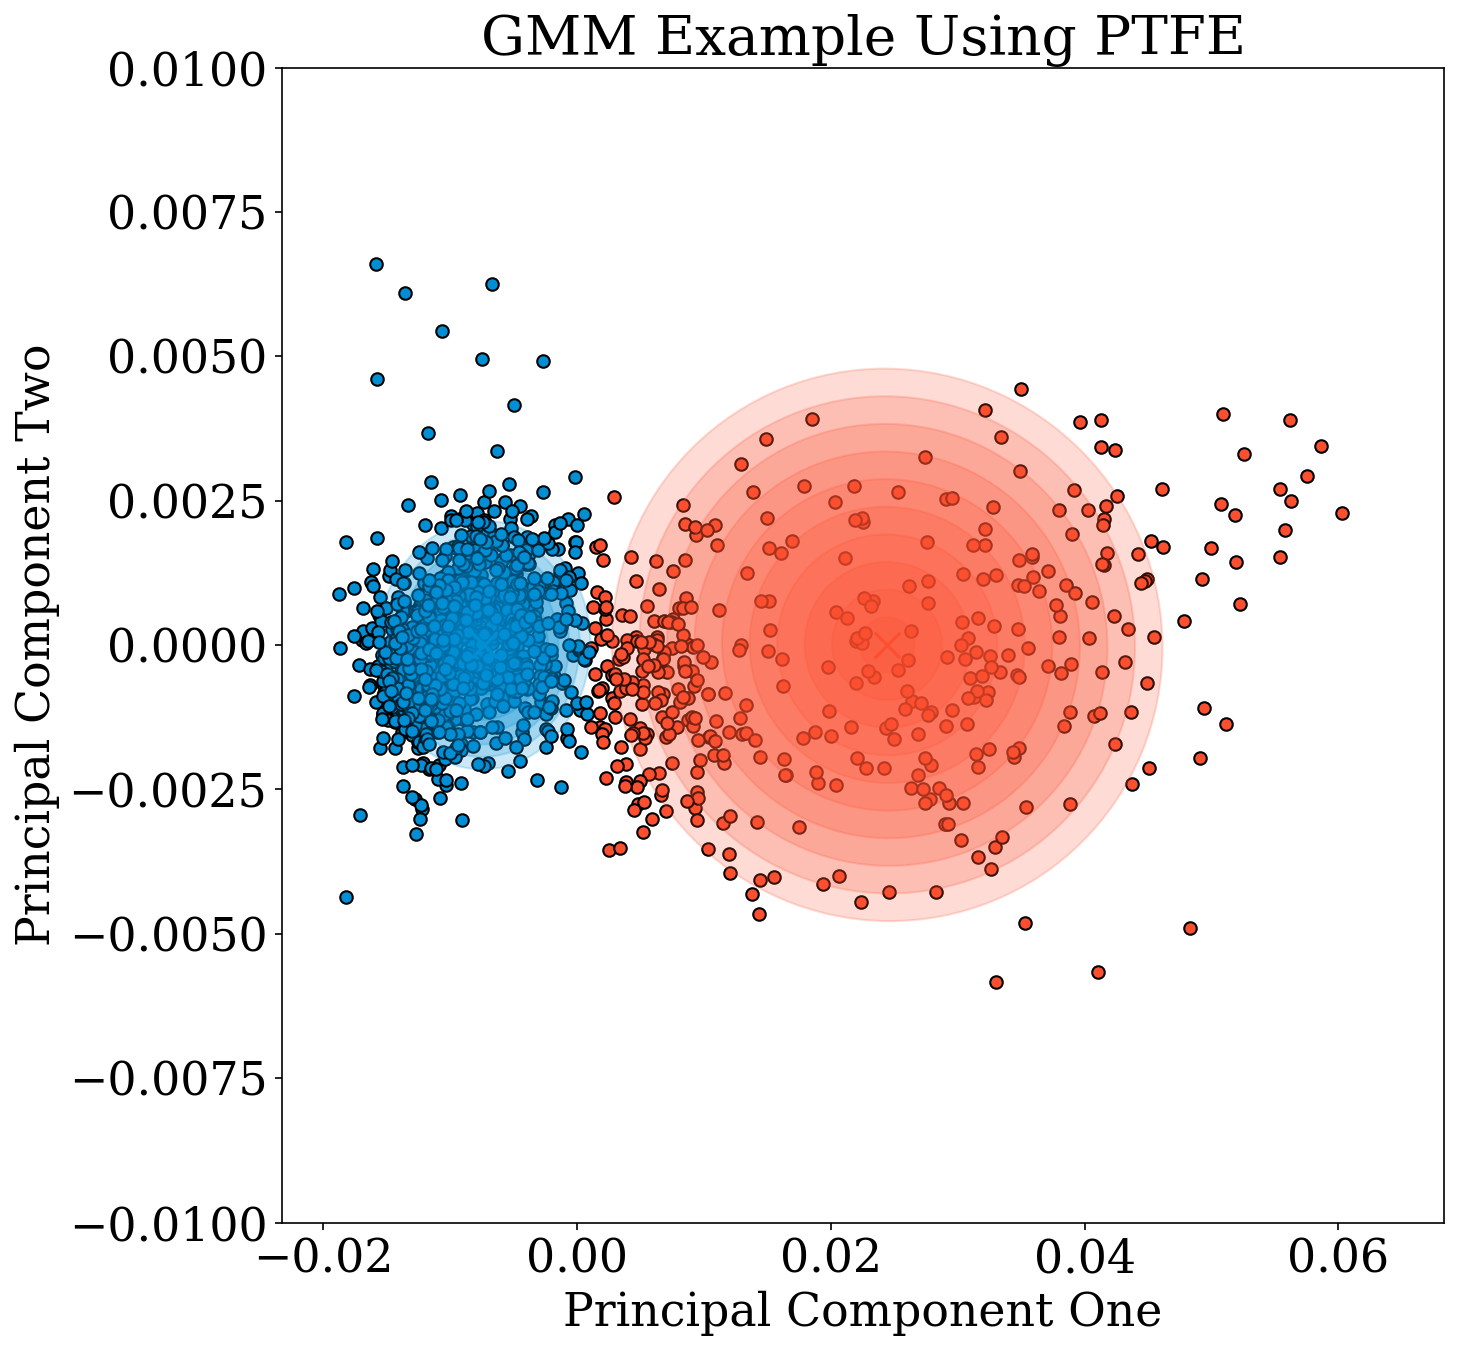
\includegraphics[width=\textwidth]{figures/GMM.png}
    \end{subfigure}

    \caption{Comparison of K-means to GMM on the polypropylene image. A contour is displayed representing the probabililty distribution for the GMM and the euclidean distance for K-means is displayed.}
    \label{clustering_methods}
\end{figure}

\subsubsection{Gaussian Mixture Models}

A gaussian mixture model (GMM) can be used as a clustering method implicitly accounts for the Gaussian nature of a dataset. We expect this method to behave well for the Poisson statistics present in imaging. First we will discuss a general mixture model and then we will see how it is changed by assuming a Gaussian distribution. A more complete overview of GMMs can be found at \cite{DinovExpectationTutorial}.

General mixture models contain $N$ data points, each assumed to be a mixture of $K$ components, with all of these components assumed to be from the same family of distributions. In this case a Gaussian distribution. However these distributions are allowed to have different parameters, in this case different means and variances. The model also includes the identity of the mixture component to which each data point belongs. Also necessary is a weighting of each of the $K$ components and sets of parameters for each of the distributions, in this case means and variances for the Gaussians. In this work the number of components used was two and a further constraint was put on the variance of the GMMs to assure that they are spherical in the PCA case.

A bayesian GMM (BGMM) differs from the regular GMM in the fitting of the statistical model to the data. A regular GMM uses the expectation maximization (EM) algorithm to fit the gaussian to the data. In a BGMM variational inference extends the EM algorithm to maximize the lower bound on model evidence (including priors) instead of the maximum likelihood \cite{Blei2006VariationalMixtures}.

\subsubsection{Other Clustering Methods}

A number of other clustering methods were compared. These additional methods and their parameters are summarized in Table \ref{tab1}.


% Please add the following required packages to your document preamble:
% \usepackage[table,xcdraw]{xcolor}
% If you use beamer only pass "xcolor=table" option, i.e. \documentclass[xcolor=table]{beamer}
\begin{table}[htbp]
\begin{tabular}{|l|l|l|l|}
\hline

Method name                                                            & Parameters                                                                                                                                         & Notes on Parameters                                                                                                                & Geometry (metric used)                                                      \\ \hline
K-Means                                                                & number of clusters                                                                                                                                 & \begin{tabular}[c]{@{}l@{}}1 or 2,\\ defined by silhouette\\ score \cite{Rousseeuw1987Silhouettes:Analysis}\end{tabular}                                                    & \begin{tabular}[c]{@{}l@{}}Squared Euclidean\\ Distance\end{tabular}        \\ \hline
Mean-shift \cite{Fukunaga1975TheRecognition}                                                             & bandwidth                                                                                                                                          & \begin{tabular}[c]{@{}l@{}}estimated using\\ scikit-learn's bandwidth\\ estimator\end{tabular}                                     & \begin{tabular}[c]{@{}l@{}}Euclidean \\ Distance\end{tabular}               \\ \hline
Spectral clustering                                                  & \begin{tabular}[c]{@{}l@{}}number of clusters,\\ eigensolver,\\ label assignment\end{tabular}                                                      & \begin{tabular}[c]{@{}l@{}}1 or 2,\\ ARPACK \cite{Lehoucq1998ARPACKMethods},\\ K-means\end{tabular}                                        & \begin{tabular}[c]{@{}l@{}}Nearest-neighbor \\ graph distance\end{tabular}  \\ \hline
\begin{tabular}[c]{@{}l@{}}Ward hierarchical\\ clustering \cite{Ward1963HierarchicalFunction}\end{tabular} & \begin{tabular}[c]{@{}l@{}}number of clusters,\\ connectivity matrix\end{tabular}                                                                  & \begin{tabular}[c]{@{}l@{}}1 or 2,\\ estimated as:\\ $1/2*(C+C')$\\ where C is the\\ K neighbors graph of\\ the data.\end{tabular} & \begin{tabular}[c]{@{}l@{}}Squared\\ euclidean\\ distance\end{tabular}      \\ \hline
HDBSCAN \cite{Campello2015HierarchicalDetection}                                                                & \begin{tabular}[c]{@{}l@{}}minimum samples,\\ minimum cluster size,\\ metric\end{tabular}                                                          & \begin{tabular}[c]{@{}l@{}}10,\\ 10,\\ minkowski\end{tabular}                                                                      & \begin{tabular}[c]{@{}l@{}}Distances between\\ nearest points\end{tabular}  \\ \hline
Gaussian Mixture                                                       & \begin{tabular}[c]{@{}l@{}}number of clusters,\\ covariance type\end{tabular}                                                                      & \begin{tabular}[c]{@{}l@{}}1 or 2,\\ spherical\end{tabular}                                                                        & \begin{tabular}[c]{@{}l@{}}Mahalanobis \\ distances to centers\end{tabular} \\ \hline
Birh \cite{Zhang1996BIRCH}                                               & \begin{tabular}[c]{@{}l@{}}number of clusters,\\ branching factor, \\ threshold\end{tabular}                                                       & \begin{tabular}[c]{@{}l@{}}1 or 2,\\ 19,\\ 0.0001\end{tabular}                                                                     & \begin{tabular}[c]{@{}l@{}}Euclidean \\ distance\end{tabular}               \\ \hline
Gaussian Mixture                                                       & \begin{tabular}[c]{@{}l@{}}number of clusters,\\ covariance type,\\ weight concentration\\ prior type,\\ weight concentration\\ prior\end{tabular} & \begin{tabular}[c]{@{}l@{}}1 or 2,\\ spherical,\\ dirichlet process,\\ 1/(number of clusters)\end{tabular}                      & \begin{tabular}[c]{@{}l@{}}Mahalanobis \\ distances to centers\end{tabular} \\ \hline
\end{tabular}
\caption{Summary of clustering methods}
\label{tab1}
\end{table}

\subsection{Metrics}
\subsubsection{V-measure}

To evaluate the effectiveness of the clustering methods a ground truth was acquired for each image. These ground truths were manually segmented with the help of a reference photograph of the phantom imaged. For clarity, the labels we give to the ground truth will be referred to as classes while the results of the clustering methods will be clusters.

Evaluation compared these ground truth classes to clusters. When comparing the clusters to the ground truth two principals were considered: The first metric is homogeneity. Homogeneity is satisfied if a cluster contains data points of a single class. We note, if using homogeneity as the sole evaluation metric, assigning all points to one class would attain a perfect evaluation score. Thus we introduce a second evaluation metric, completeness, satisfied if all data points of a single class are in a single cluster. 

Homogeneity and completeness are formulated mathematically using the method described by Rosenberg and Hirschberg \cite{Rosenberg2007V-Measure:Measure} which can be found in the Appendix. To simplify we build a single metric that uses a combination of both homogeneity $h$ and completeness $c$. This combination is called the V-measure and is the harmonic mean of homogeneity and completeness.


\begin{equation}
v = 2 \cdot \frac{h \cdot c}{h + c}
\end{equation}

This value ranges from 0 to 1, a perfect classification has a score of one while assigning each point to a cluster would result in a score of zero.

\subsubsection{Akaike Information Criterion}

The Akaike information criterion (AIC) \cite{Akaike1998InformationPrinciple} is an estimator of the relative quality of a statistical model for a given data set. Unlike a V-measure, AIC could not compare different clustering methods, and was used instead to find parameters for the GMMs. As most clustering models discussed do not include a statistical models it's application is limited to the GMMs.

AIC is a function of the goodness of fit of a statistical model combined with a penalty for overfitting. In this work AIC tested the goodness of fit of the GMM's Gaussian, with a penalty proportional to the number of clusters. Used this way, AIC determines can determine the optimal number of clusters and other GMM parameters.

Specifically the maximum likelihood found while fitting the GMMs using the EM algorithm, $\hat L$, and the number of parameters $k$ were used to calculate the AIC as:

\begin{equation}
    AIC \, = \, 2k - 2\ln(\hat L)
\end{equation}

For a given model the lowest AIC denotes a better fit. More specifically an "elbow" or change in curvature of the AIC as a function of the number of components denotes the optimal number of components. For BGMMs, which do not produce a maximum likelihood in training, AIC was calculated using the $\hat L$ from a GMM with the same parameters.

\subsubsection{Interpolating Bayesian Gaussian Mixture Model}

%Initial clustering results contained many pixels misclassified due to poor detector response, noise in the data and partial volume effects. To combat these effects a
Additional to the previous methods, a new clustering method was also proposed. The workflow of this method is seen in Figure \ref{iterative_method} c). A BGMM was trained as in the GMM section above. Within each cluster the mahalanobis distance \cite{Mahalanobis1936OnStatistics} from all the points to the center was calculated. Points greater than \%90 of the maximum were then identified as potential outliers. Each potential outlier was then interpolated spacialy using biharmonic interpolation \cite{Damelin2017OnAspects}. The BGMM was then retrained using starting point defined by the end state of the previous iteration. The process was then repeated until convergence. Convergence was indicated when the AIC of the model increased. In practice this amounted to between five and ten iterations. A demonstration of this method can be seen in Figure \ref{iterative_method} a-b).

\begin{figure}[htbp]
    \centering
    \begin{subfigure}[b]{0.48\textwidth}
        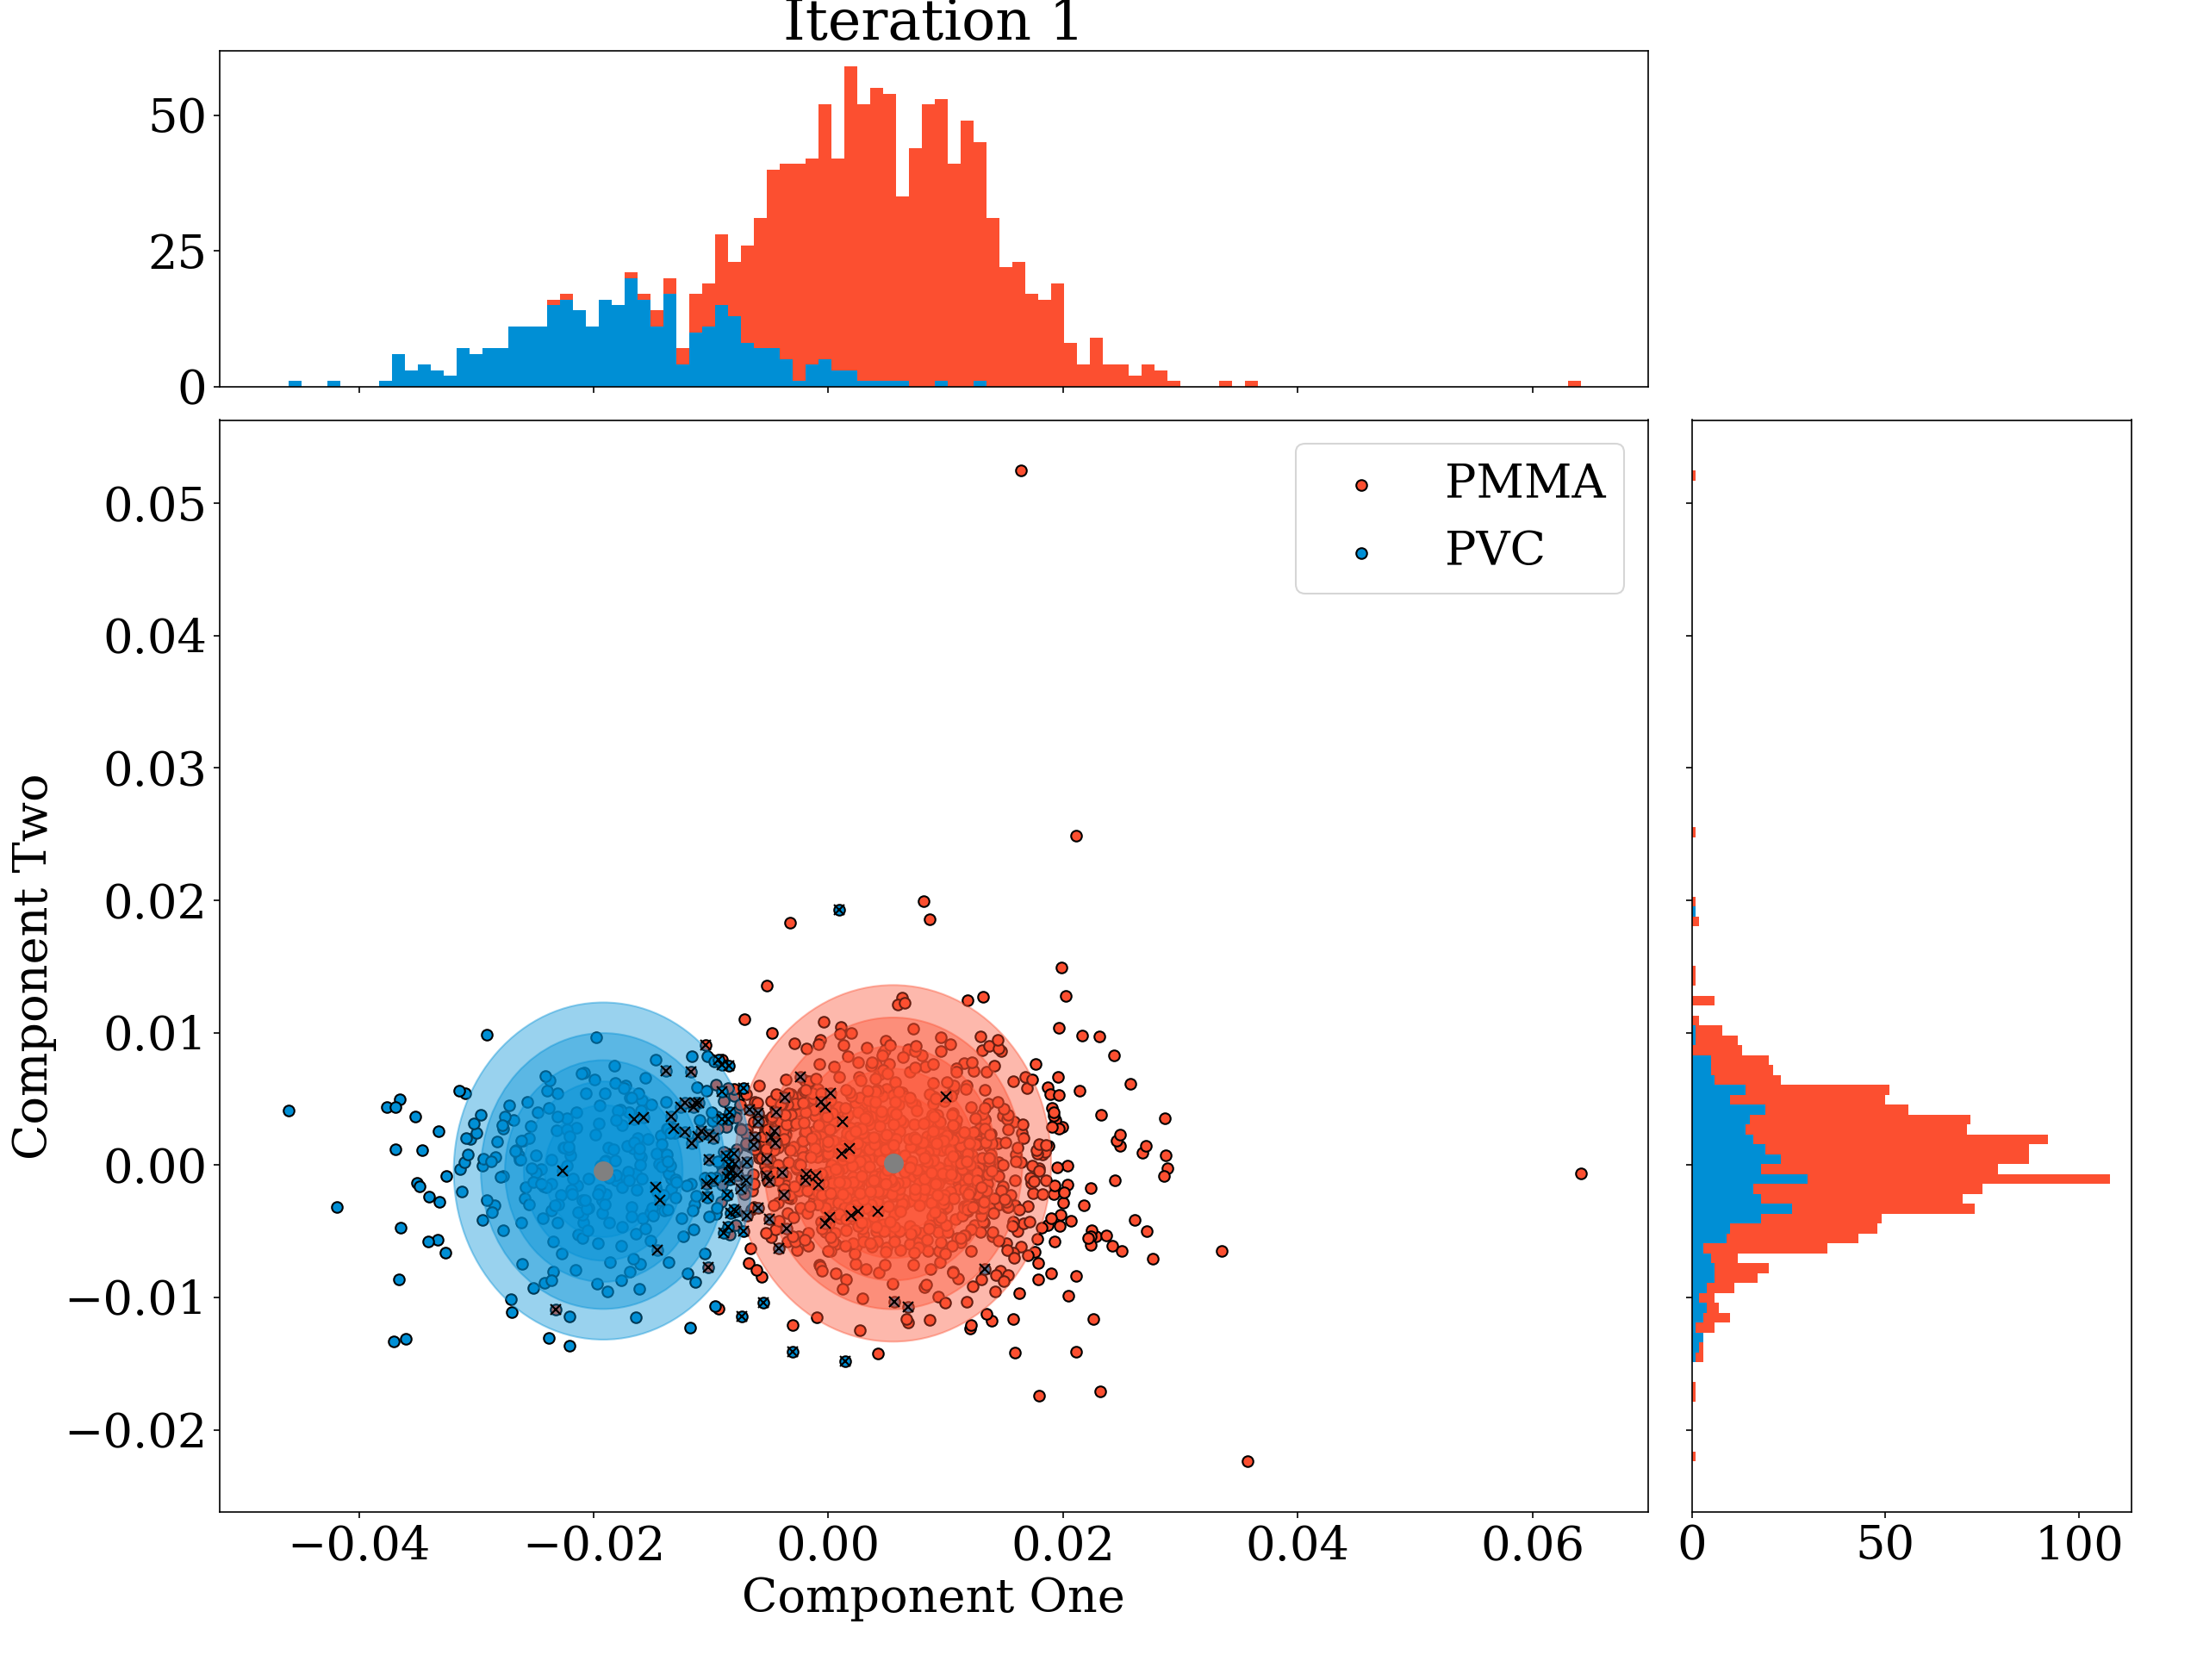
\includegraphics[width=\textwidth]{figures/PCAsphericalbefore.png}
    \end{subfigure}
    ~ %add desired spacing between images, e. g. ~, \quad, \qquad, \hfill etc. 
      %(or a blank line to force the subfigure onto a new line)
    \begin{subfigure}[b]{0.48\textwidth}
        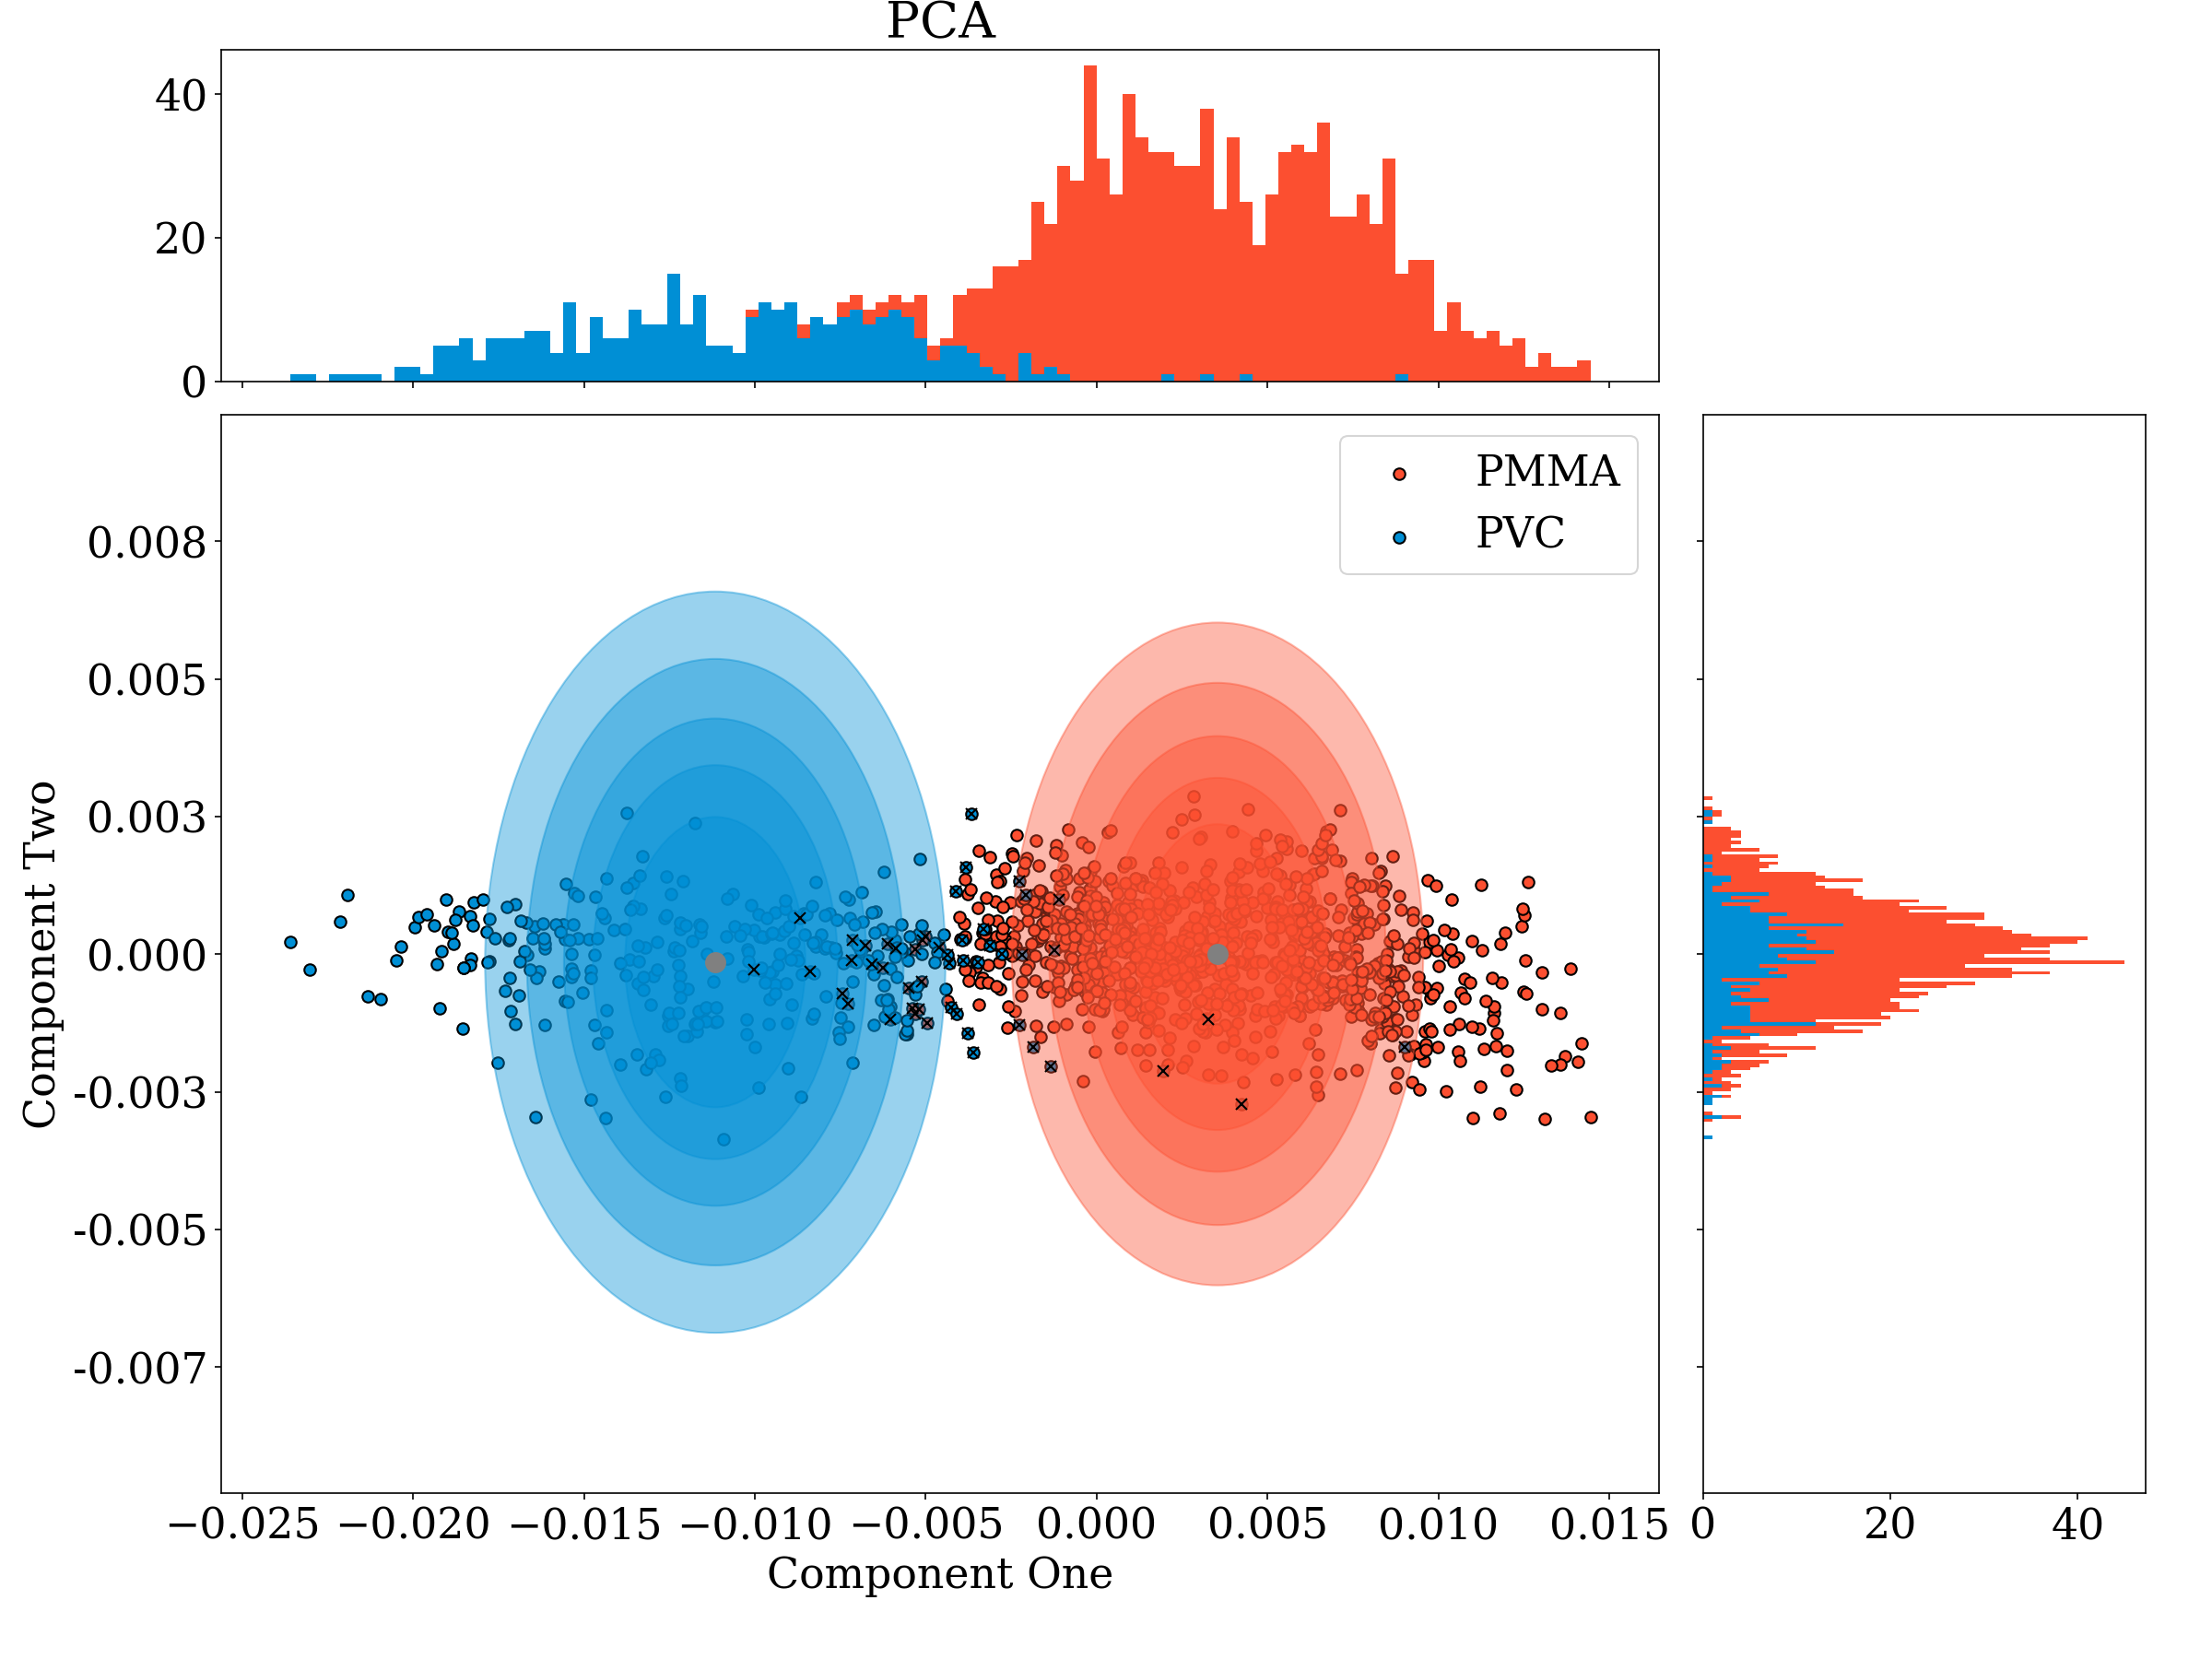
\includegraphics[width=\textwidth]{figures/PCAsphericalafter.png}
    \end{subfigure}
    \caption{IBGMM method. The left plot shows the original PVC clustering using the BGMM. The middle plot shows the final clustering after convergence.}
    \label{iterative_method}
\end{figure}

\begin{wrapfigure}{R}{0.5\textwidth}
  
  \begin{center}
    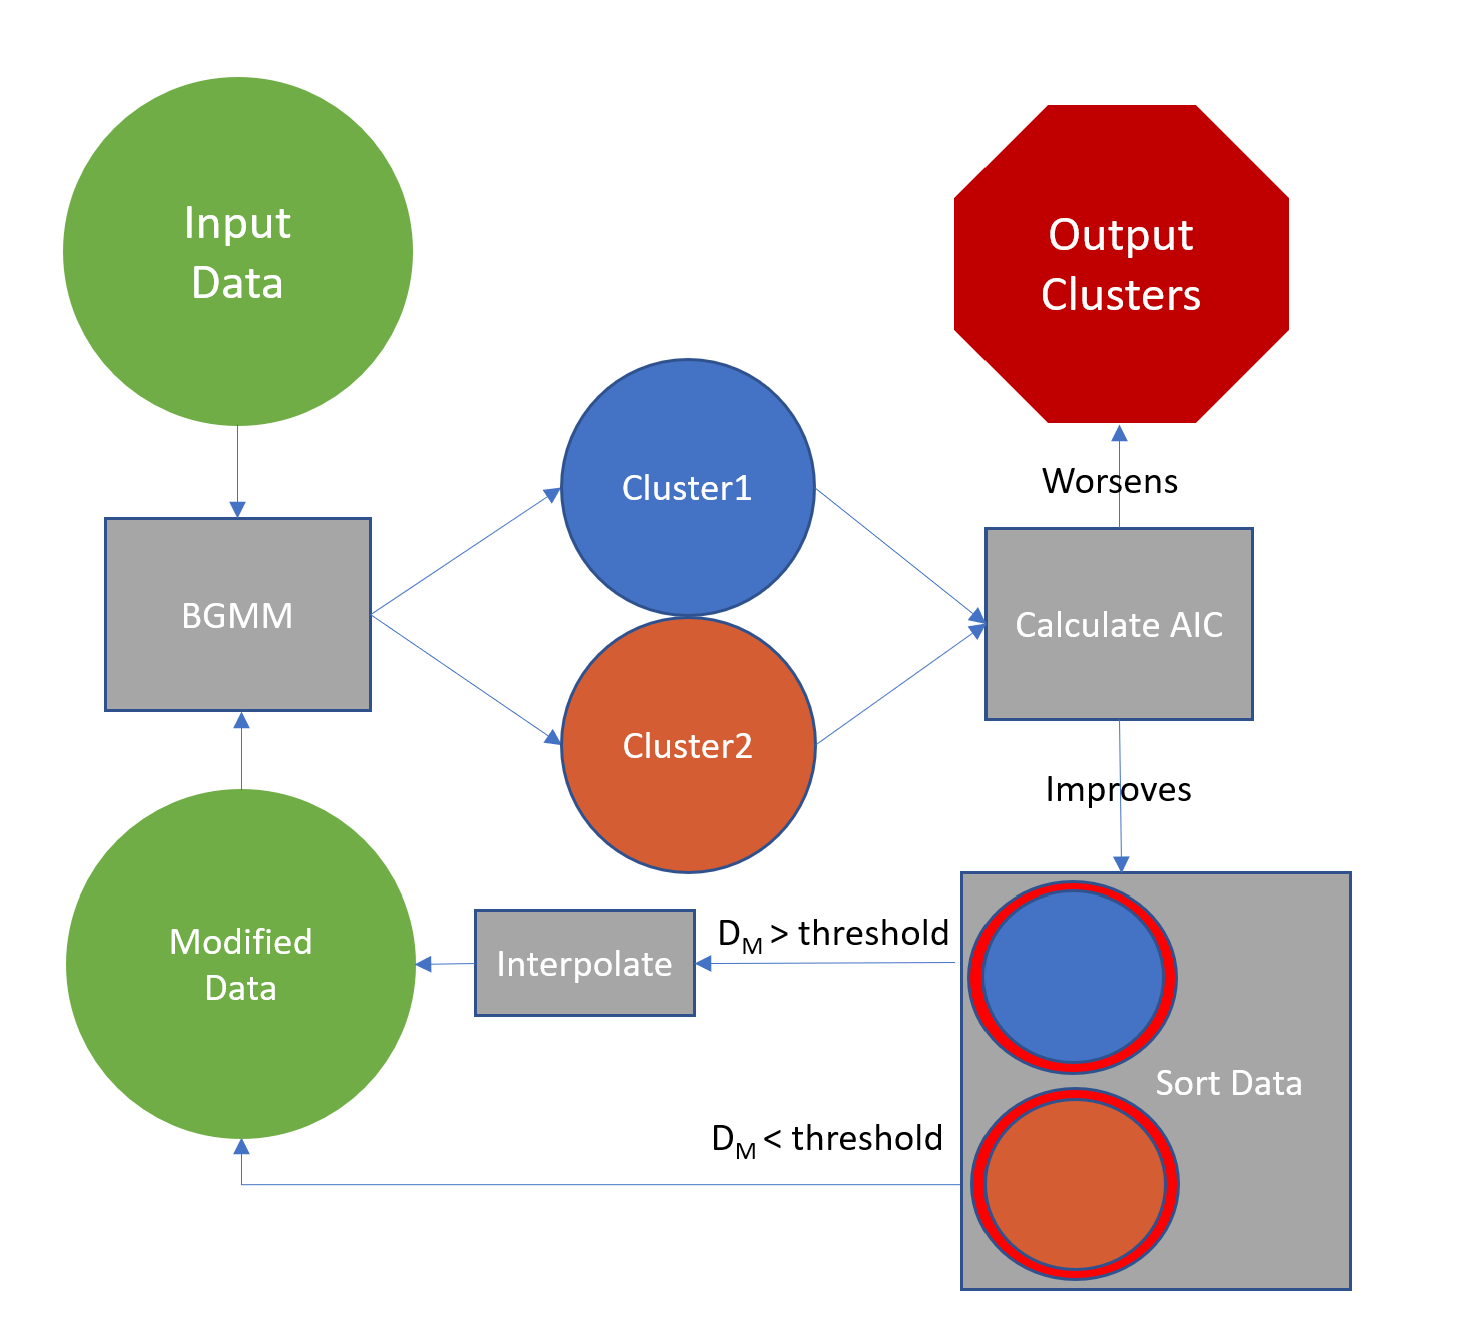
\includegraphics[width=0.48\textwidth]{figures/algo_flow.png}
  \end{center}
  
    \caption{An overview of the workflow.}
  
  \label{algo_flow}
\end{wrapfigure}

\subsubsection{Post-processing}

The aim of this work is to entirely automate image segmentation. Thus on top of the clustering it is necessary to introduce an identification layer. This layer took the segmented image after the clustering and identified if there are two materials present. To do this the following framework was developed:

First a uniform filter is applied to the image so that the binary data becomes continuous. This acts to reduce the score of single pixels that have been identified. Secondly, we apply a threshold to the image of 0.2. Next, we fill all of the binary holes in the image to make candidates for segmentation more uniform. A bounding box is then created around all of the nonzero elements of the image and overlaid on the image as the final output.




%--------------------------------------------------------------------------------%
%%%%%%%%%%%%%%%%%%%%%%%%%%%%%% Results %%%%%%%%%%%%%%%%%%%%%%%%%%%%%%%%%%%%
%--------------------------------------------------------------------------------%

\section{Results and Discussion}

\subsection{Dimensional Reduction Results}

\subsection{Clustering Results}

\begin{wrapfigure}{R}{0.48\textwidth}
  
  \begin{center}
    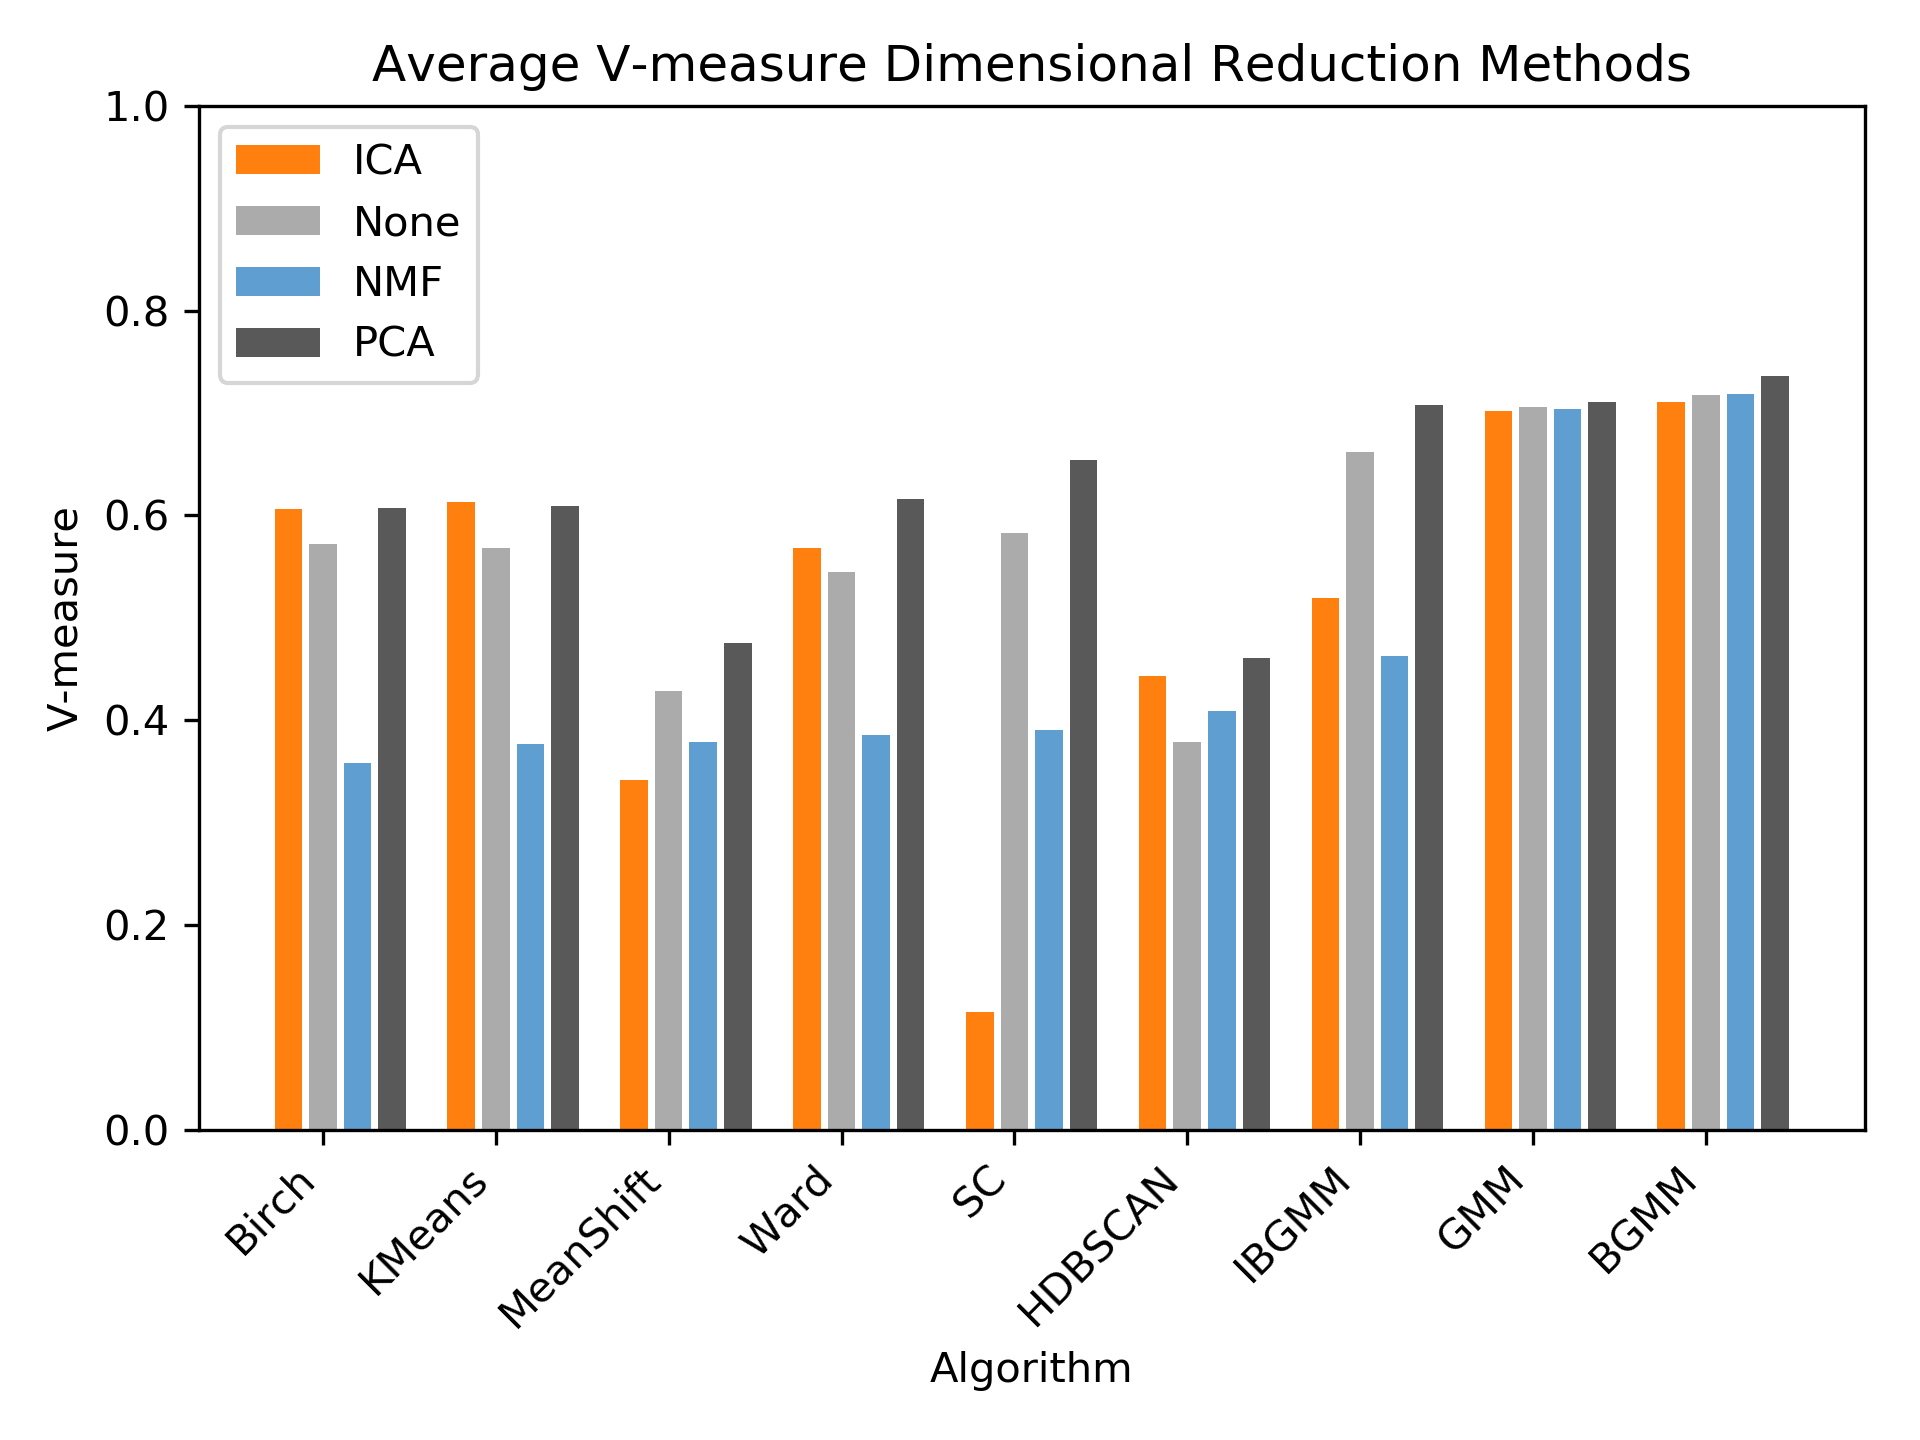
\includegraphics[width=0.48\textwidth]{figures/red_methods.png}
  \end{center}
  
  \caption{Dimensional reduction results}
  
  \label{results:dr}
\end{wrapfigure}

Figure \ref{results:dr} shows the V-measures for different dimensional reduction methods averaged over all materials for each clustering method. The dimensional reduction methods reduced the dimensionality from five to two in each case. For comparison the results without dimensional reduction are also displayed.

Overall PCA had the best results combined with the BGMM. V-measures were 0.71, 0.72, 0.72, and 0.74 for ICA, no dimensional reduction, NMF, and PCA respectively. PCA was on average 2.7\% better than ICA and 2.6\% better than NMF in this case. All other clustering methods performed the best with PCA other than K-means which performed better with ICA.

% Figure \ref{results:hard_soft} a) shows the results of the clustering methods using PCA with two principal components. Overall the GMMs resulted in the best clustering V-measures. Spectral clustering resulted in comparable V-measure in some cases.

\begin{figure}[b!]
    \centering
    \begin{subfigure}[b]{0.32\textwidth}
        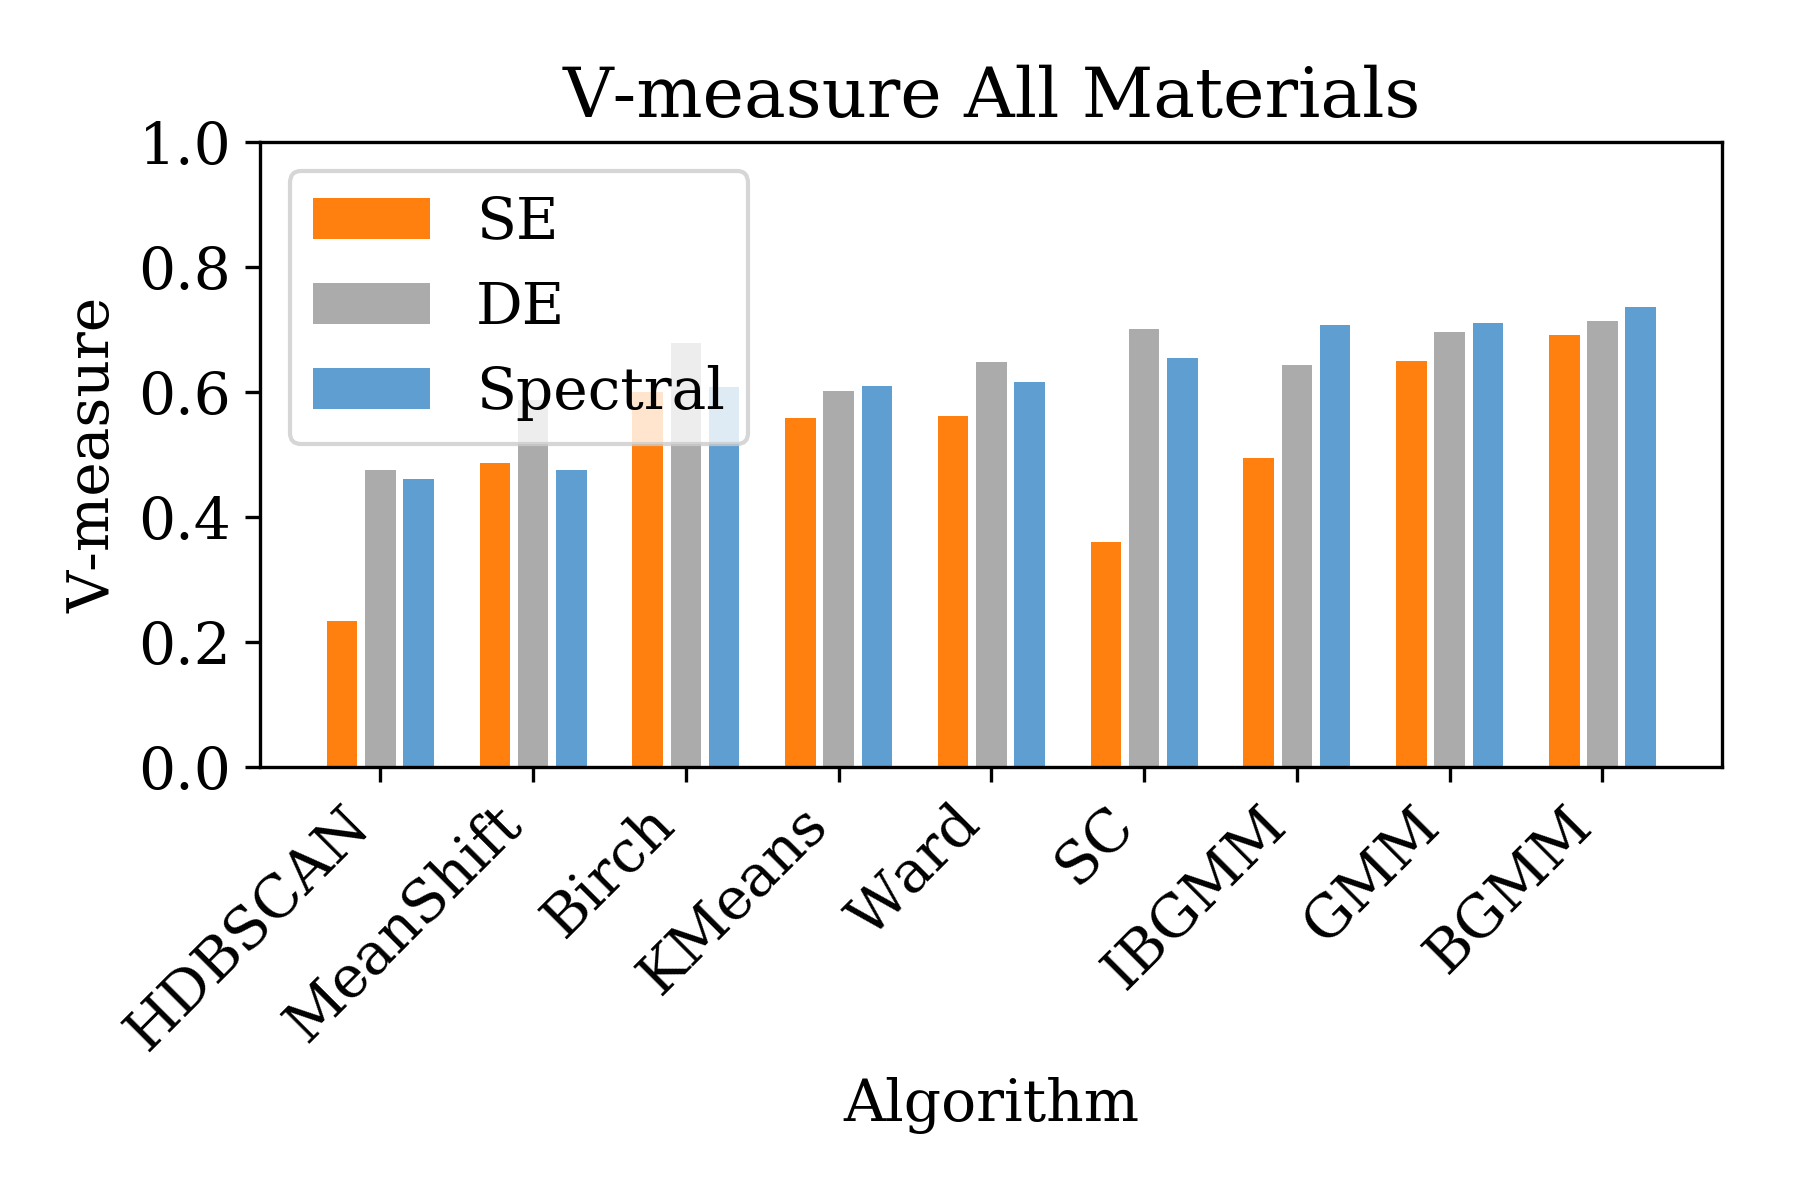
\includegraphics[width=\textwidth]{figures/energy_comparison.png}
    \end{subfigure}
    ~ %add desired spacing between images, e. g. ~, \quad, \qquad, \hfill etc. 
      %(or a blank line to force the subfigure onto a new line)
    \begin{subfigure}[b]{0.32\textwidth}
        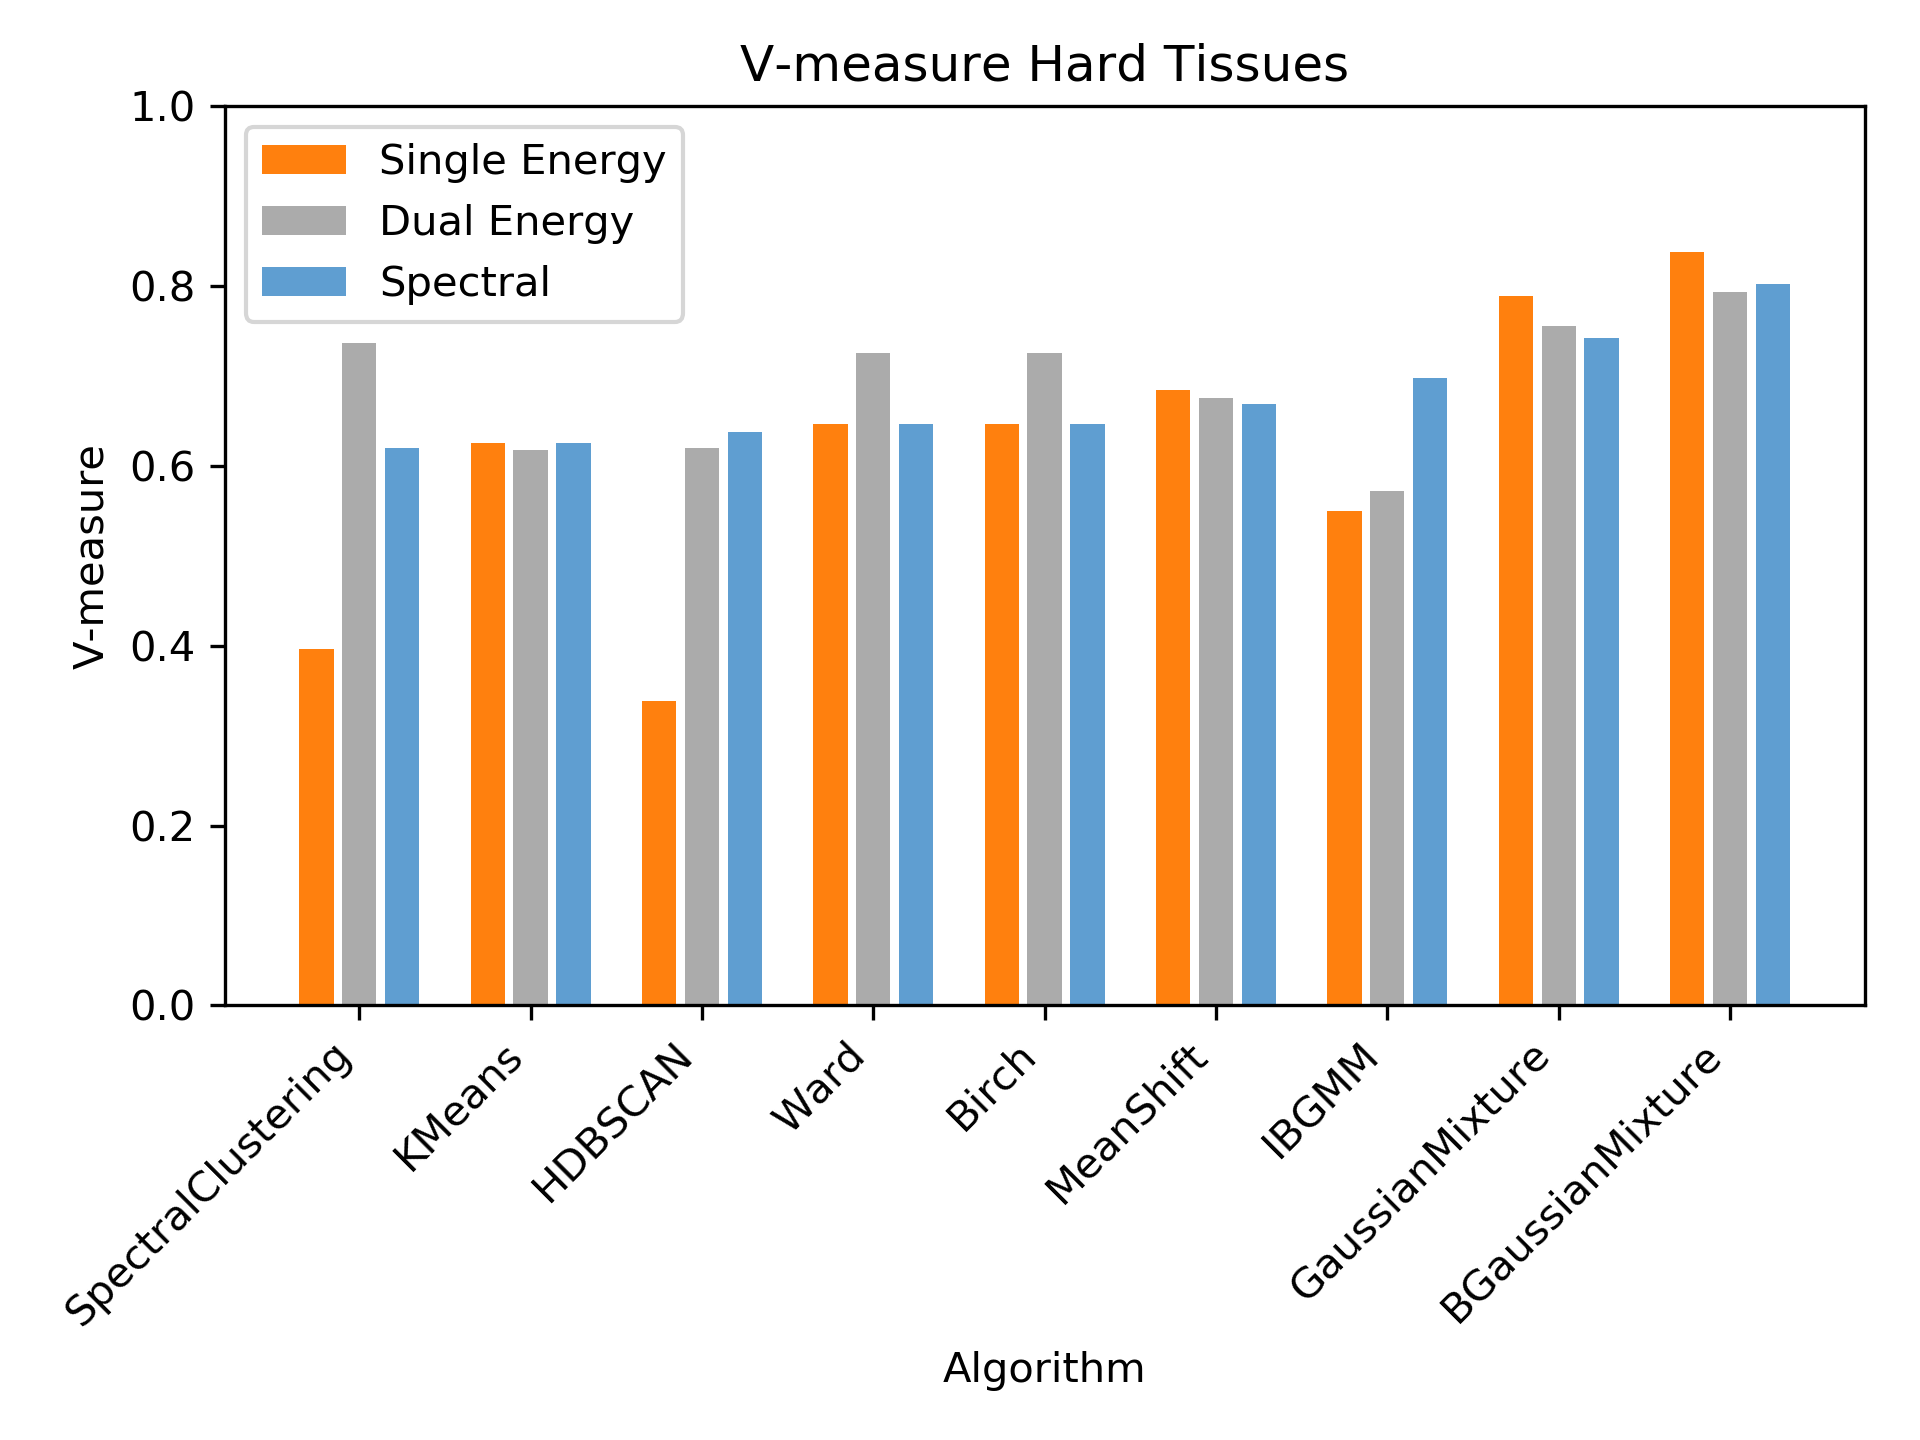
\includegraphics[width=\textwidth]{figures/hard.png}
    \end{subfigure}
    \begin{subfigure}[b]{0.32\textwidth}
        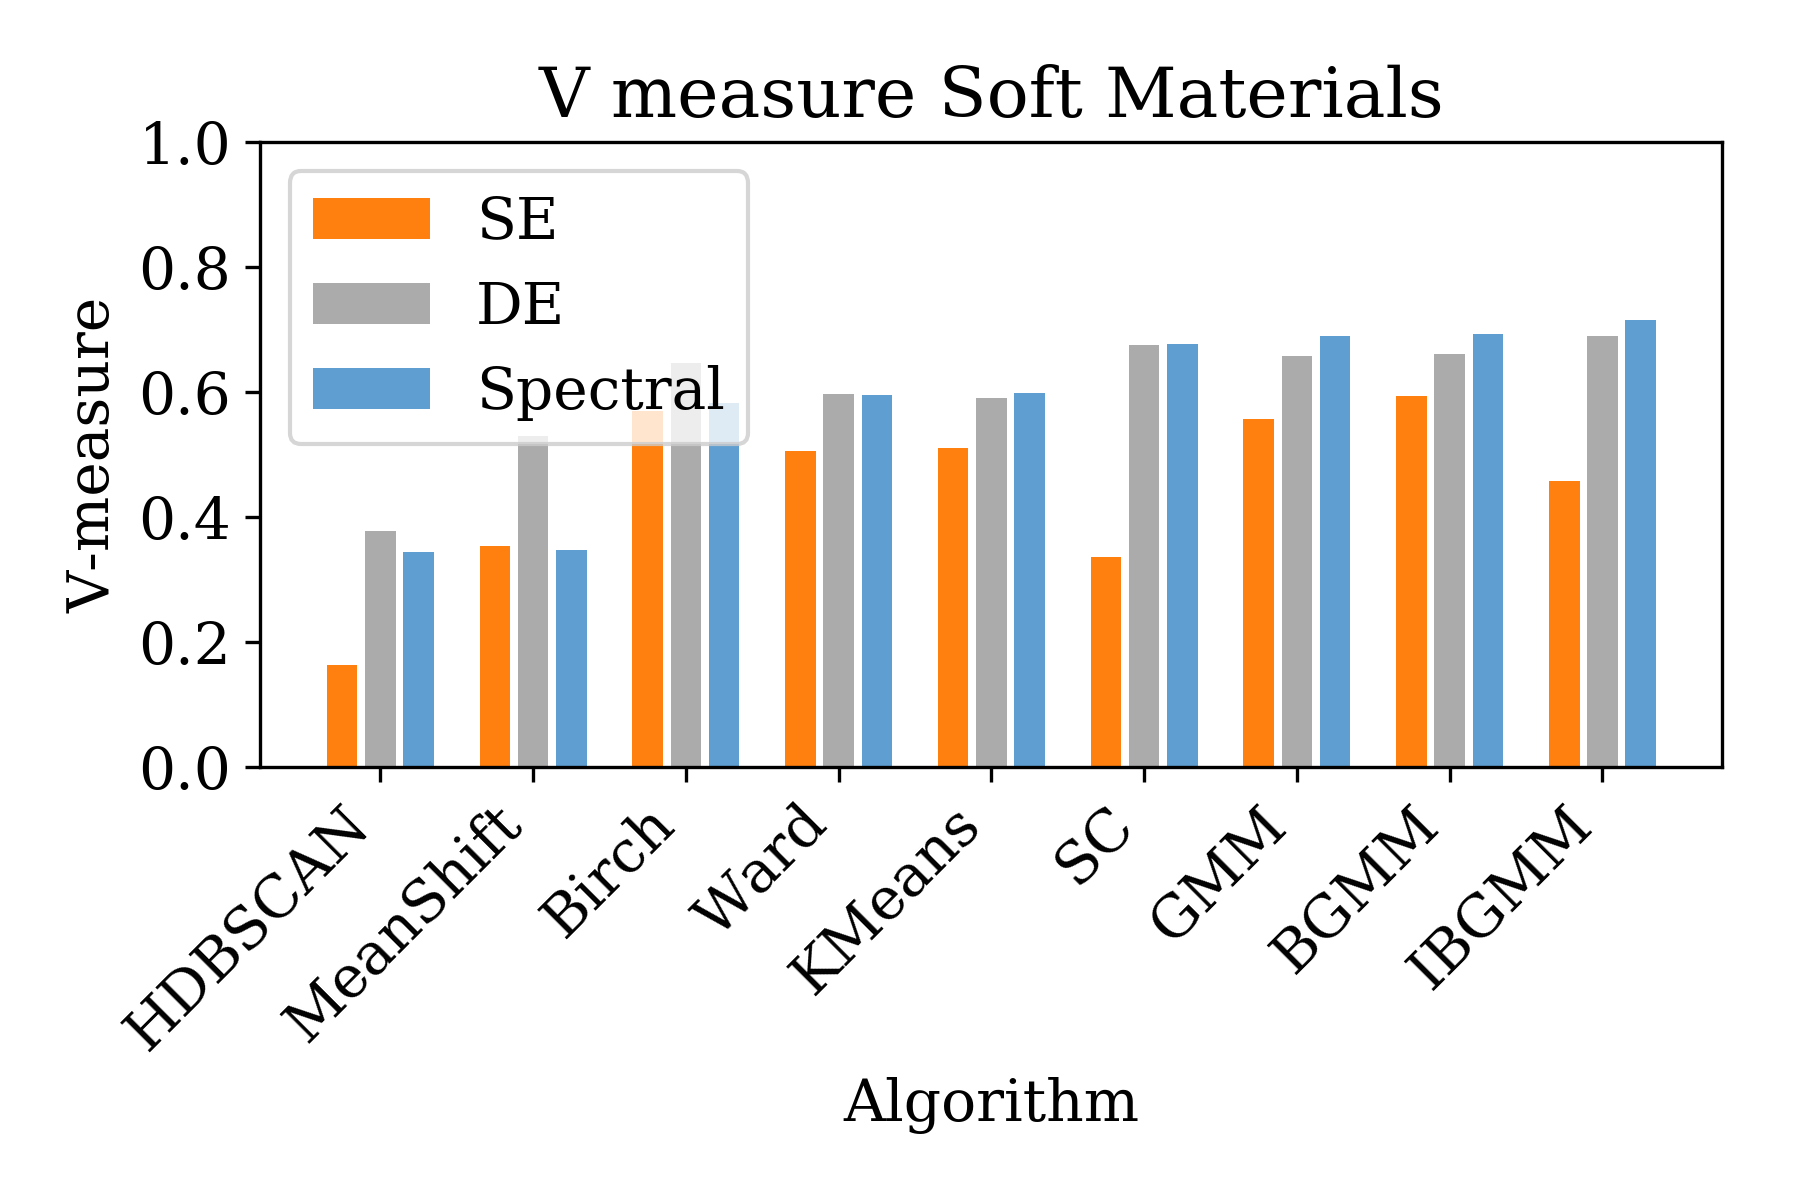
\includegraphics[width=\textwidth]{figures/soft.png}
    \end{subfigure}
    \caption{Comparison to Dual and Single Energy using V-measure with results averaged over all of the tissues, soft tissues and hard tissues respectively}
    \label{results:hard_soft}
\end{figure}

\subsubsection{Single, Dual, and Spectral Comparison}

Results can be seen in Figure \ref{results:hard_soft}. Overall spectral imaging was seen to be marginally better that dual and single energy imaging averaged over all of materials. The V-measure for the BGMM method which was best in all modalities was 0.69, 0.71, and 0.74 for single, dual, and spectral respectively. Spectral was seen to be on average 4.2\% better than DE imaging and 7.2\% better than SE imaging.

Figure \ref{results:hard_soft} b-c) show the results separated in term of the material density. Hard materials such as glass and steel had the best results for SE clustering with the BGMM. The best V-measures for the hard tissues were 0.84, 0.79, and 0.80 for single, dual, and spectral respectively. While for soft materials (PVC, PTFE, PP) the IBGMM method saw the best results when clustering with spectral and DE imaging with V-measures of 0.71 and 0.69 respectively, while for SE the BGMM performed best with a V-measure of 0.59. This was a gain of 16.9\% between single and dual and a gain of 3.5\% between dual and spectral.

\subsubsection{Number of Clusters}

Given the result that BGMMs result in the lowest V-measure, there is further analysis necessary to determine if the process can be automated. Namely if we can determine the number of clusters $k$ reliably without human oversight. This was attempted by comparing the AICs and weights for both the $k=1$ and $k=2$ cases. If the AIC did not decrease significantly between one and two clusters and the weights for the two clusters were similar this indicated that there was only one material present.

The results for the multi-material phantom as well as for a blank scan of PCA are shown below. The AIC for all of materials was seen to decrease by on average 6683 and 1208 in the worst case. For the blank scan the AIC was seen to decrease by 160. The weights for the different materials were seen to be in the most equal case \%40 different for PTFE and was only \%10 different in the one material case.

\begin{figure}[b!]
    \centering
    \begin{subfigure}[b]{0.48\textwidth}
        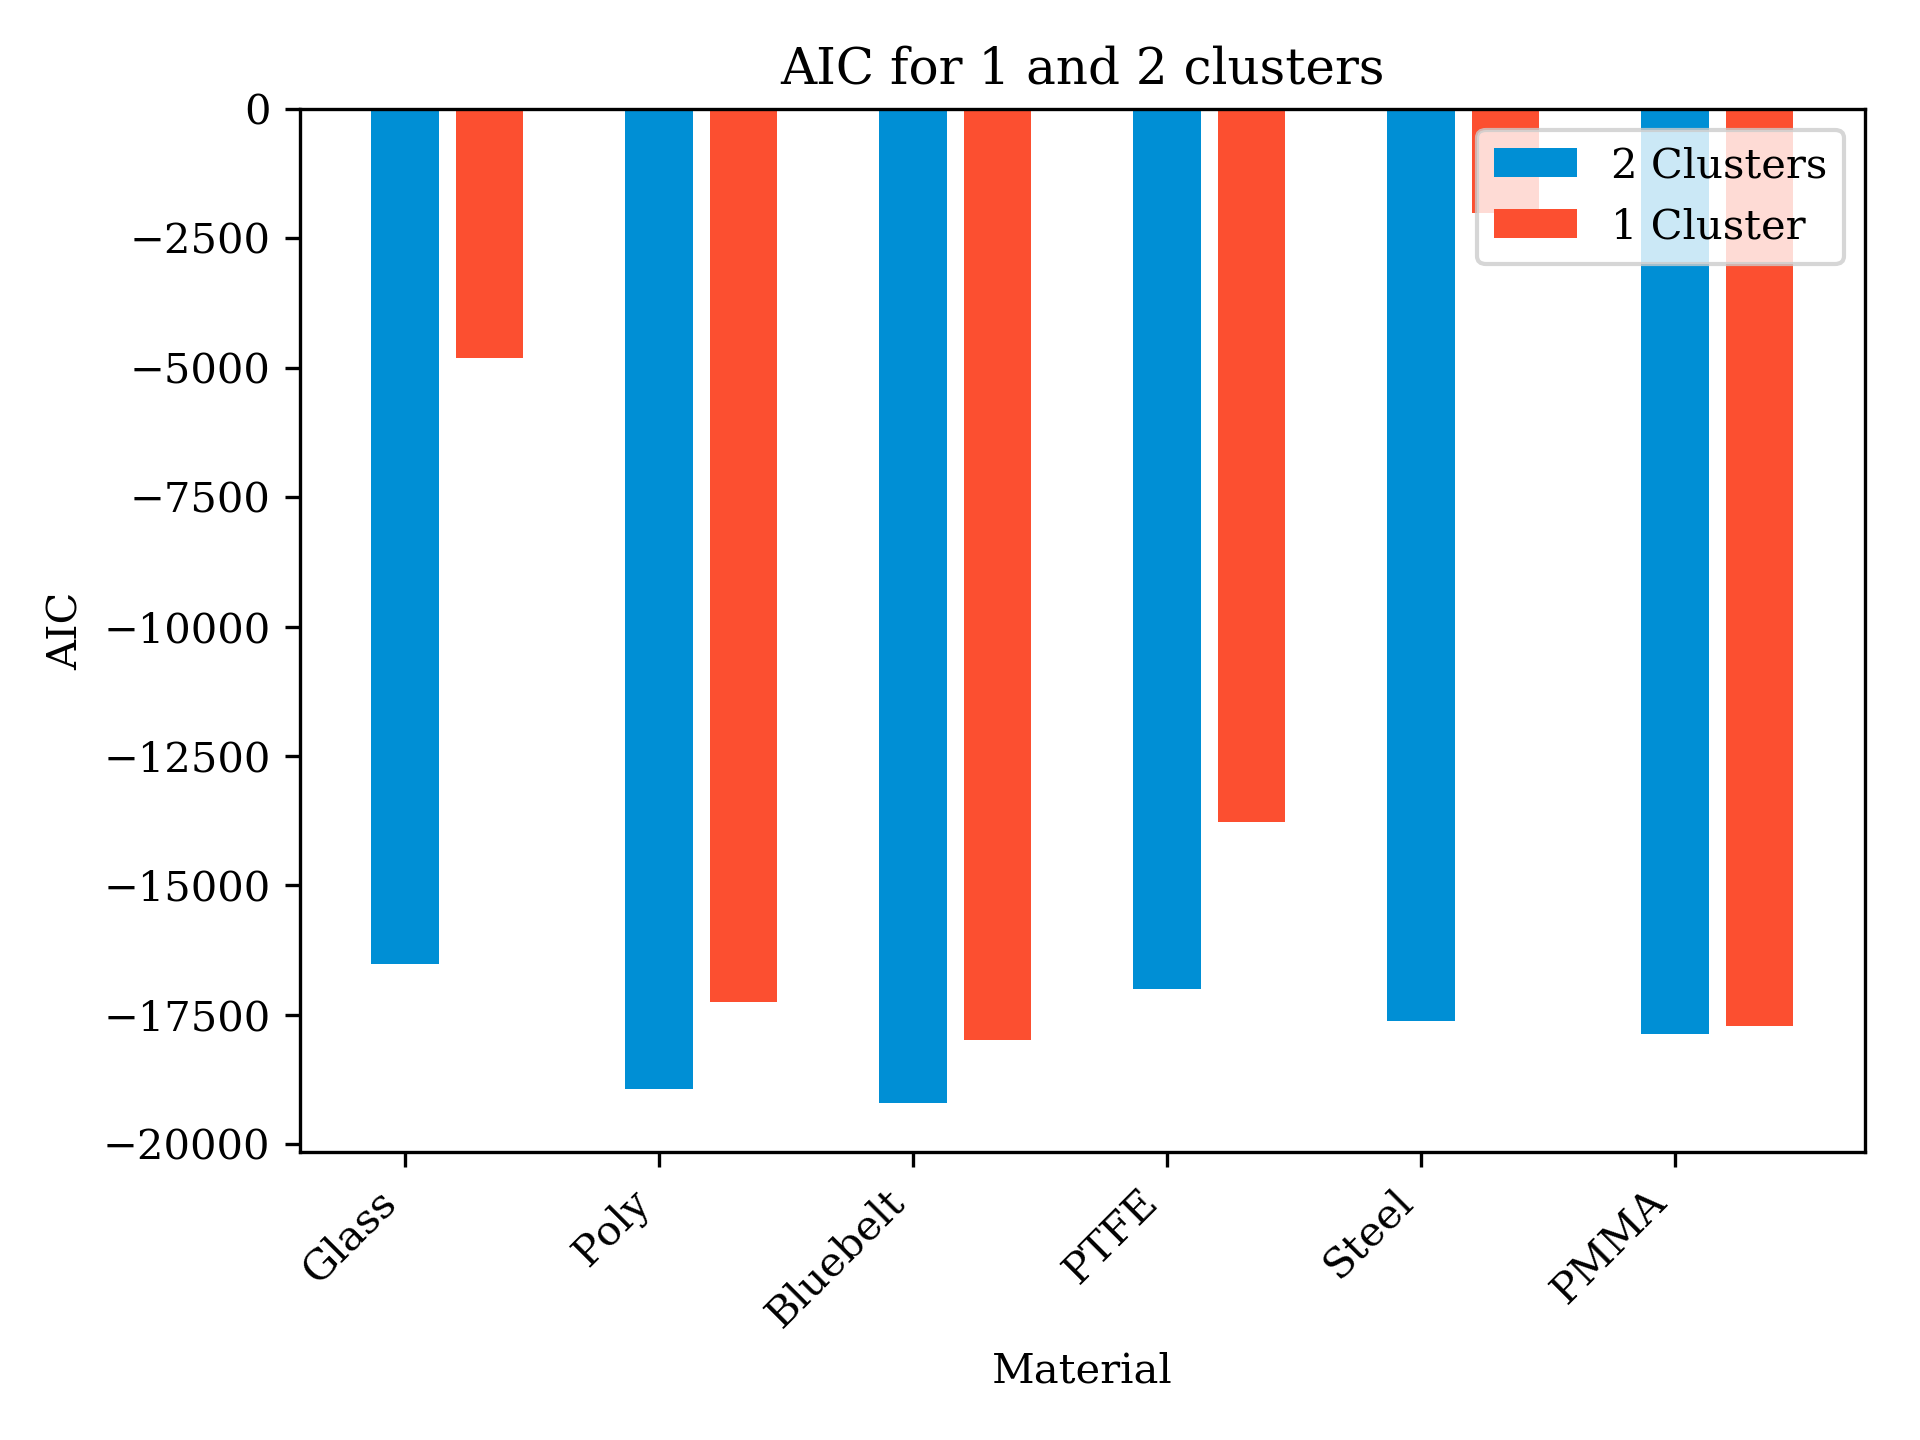
\includegraphics[width=\textwidth]{figures/AIC.png}
    \end{subfigure}
    \begin{subfigure}[b]{0.48\textwidth}
        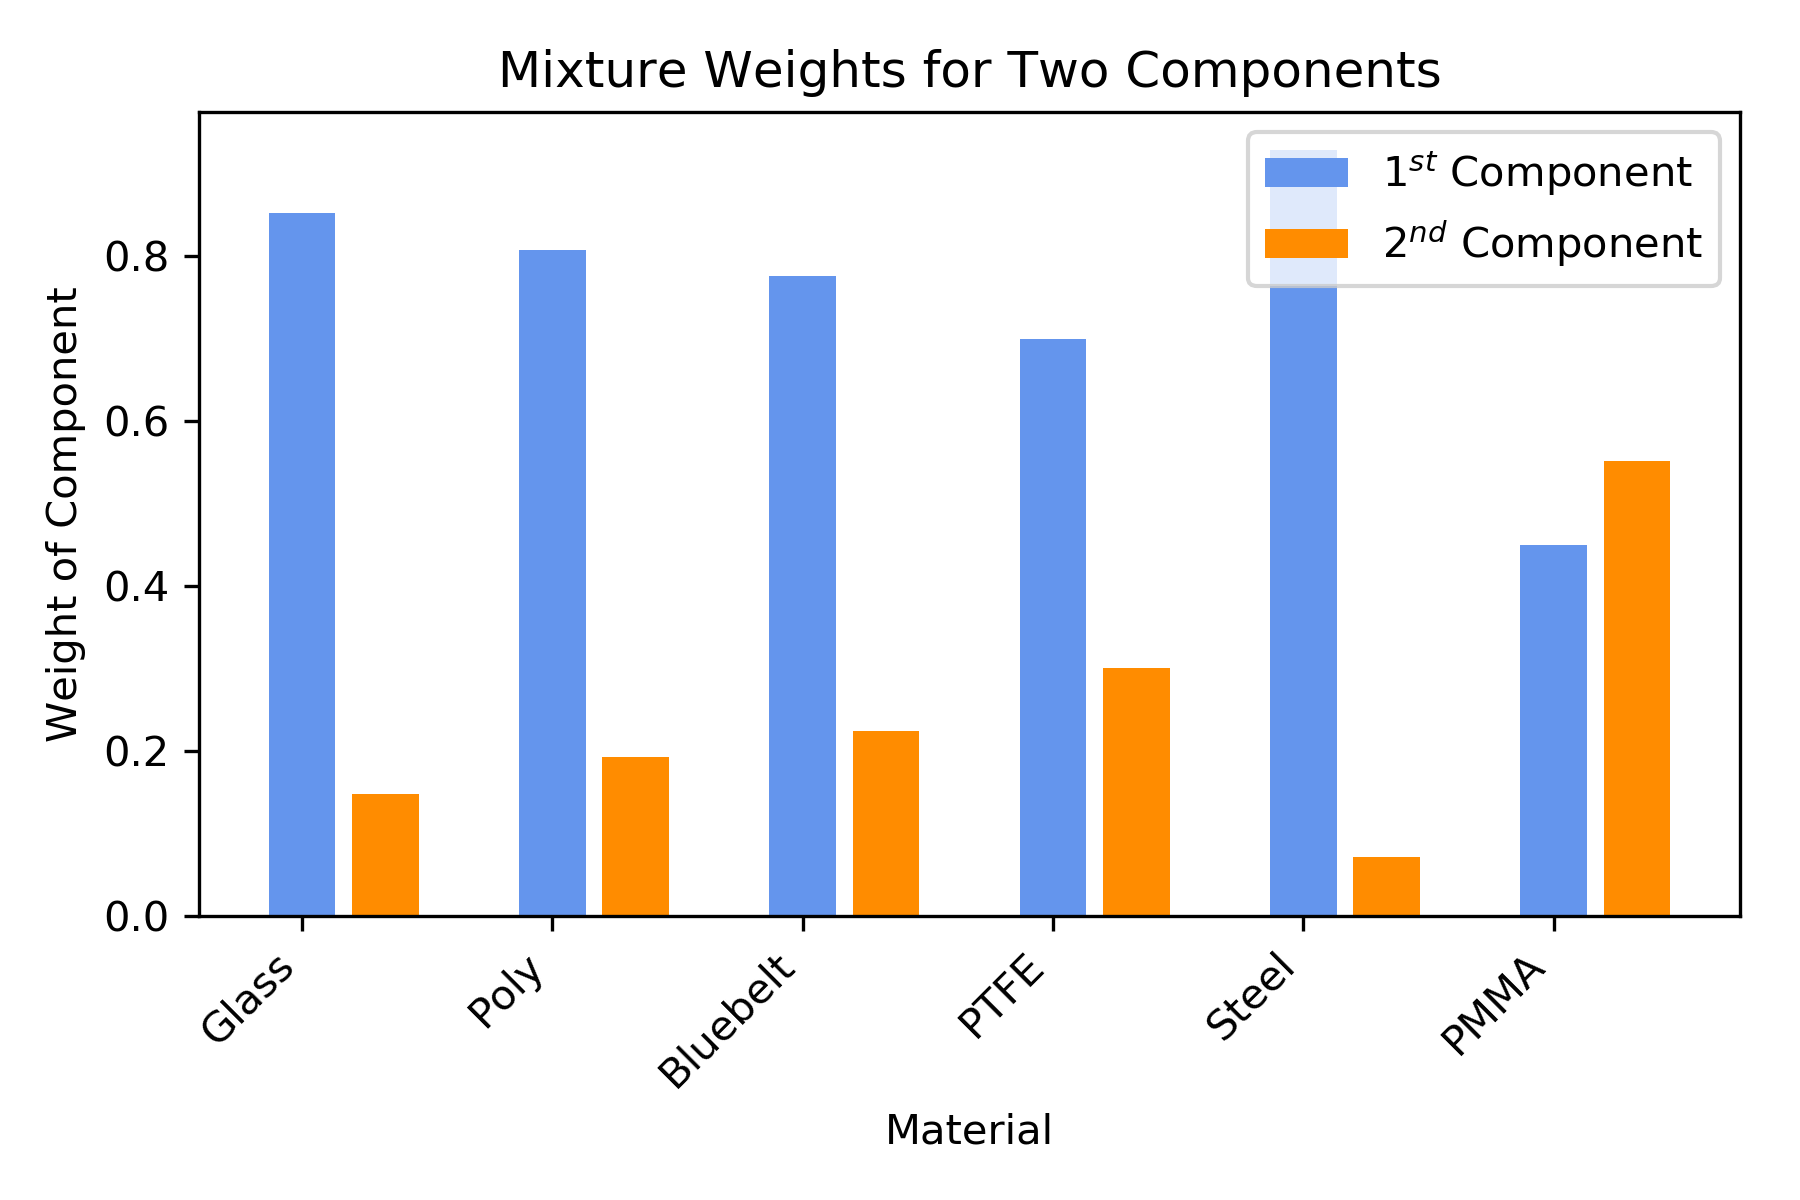
\includegraphics[width=\textwidth]{figures/weights.png}
    \end{subfigure}
    \caption{Clustering Methods}
    \label{n_bins}
\end{figure}

\subsubsection{Comparison to Otsu Thresholding}

\begin{wrapfigure}{R}{0.33\textwidth}
  
  \begin{center}
    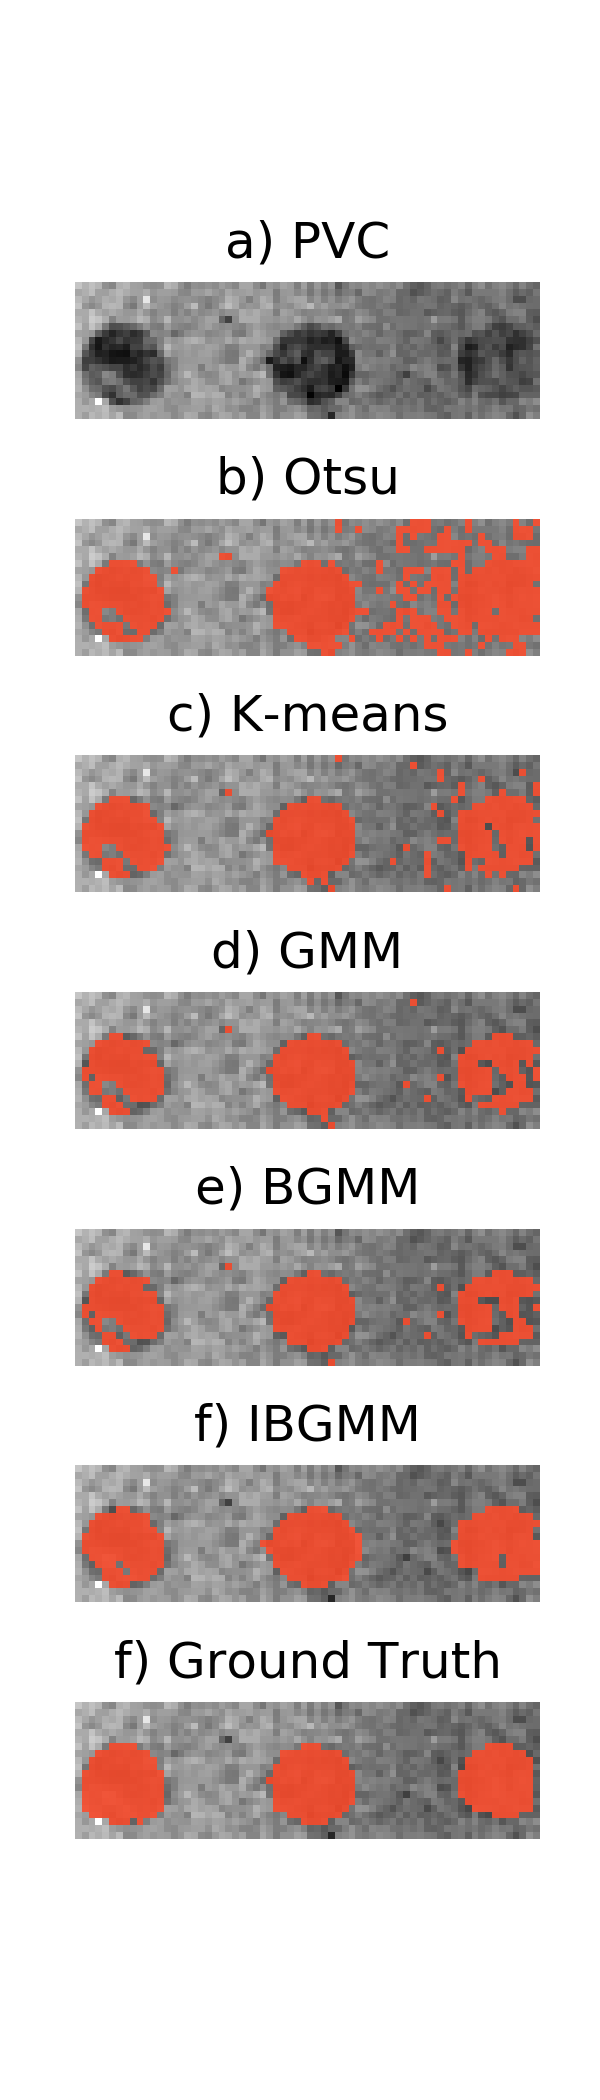
\includegraphics[width=0.33\textwidth]{figures/otsu.png}
  \end{center}
  
  \caption{Overlay of the different segmentation methods on the PVC SE image}
  
  \label{results:otsu}
\end{wrapfigure}

In X-ray image segmentation Otsu's method \cite{Otsu1979AHistograms} is sometimes used for image segmentation \cite{Sund2003AnImaging}. Here we compare this algorithm to the IBGMM with spectral imaging on a soft tissue segmentation. As can be seen in Figure \ref{results:otsu} when the background had similar composition to the material in question there was erratic thresholding of the background. In this case the IBGMM had a V-measure of 0.74 while the thresholding method has a score of 0.41. One can see in Figure \ref{results:otsu} that thresholding cannot resolve the thinnest insert in the image and the IBGMM is the only method that is able to recover the circular shape of the insert while suppressing noise in the data.


%--------------------------------------------------------------------------------%
%%%%%%%%%%%%%%%%%%%%%%%%%%%%%% Discussion %%%%%%%%%%%%%%%%%%%%%%%%%%%%%%%%%%%%
%--------------------------------------------------------------------------------%

\section{Discussion}

Spectral imaging was seen to have a 20.3\% higher V-measure than single and 3.5\% higher V-measure than DE imaging in segmenting on soft materials. Conversely, SE imaging was more effective by both dual and spectral imaging on the hard tissue segmentation with a margin of 6.3\% and 5.0\% respectively. These results are consistent with results from spectral CT. Lalonde \cite{Lalonde2016ACT} found that having three energies with would improve errors in elemental composition calculations, but only marginally compared to the gains between single and dual energy. Reaching the conclusion that DE CT is worthwhile for elemental composition calculations. Likewise in this application, SE imaging is seen to be much less effective than DE imaging for soft material segmentation while dual and spectral have similar results with spectral having a 3.5\% higher V-measure. This raises the question as to if spectral or DE imaging are ideal for this application? Moreover, are the considerable downsides of spectral and DE imaging are worth the potential benefits?

Spectral detectors currently are very expensive compared to integrating detectors. Additionally, to the best of the authors knowledge clinical implementations of CZT detectors are not available. Some DE clinical implementations are available but are expensive compared to integrating detectors. To validate the benefit for the additional cost, one would need an application that has a high throughput, requires a small detector, and needs an accurate segmentation of soft tissues. A potential candidate that fits these requirements would be mammography, since mammography machines have high throughput, image a relatively small area and aim to segment soft tissues. 

This work discusses unsupervised methods for computer vision, recently supervised methods have produced superior results to unsupervised methods in many areas such as brain segmentation \cite{Bakas2018IdentifyingChallenge}, and general tumor segmentation \cite{MedicalDecathlon}. Therefore we ask; why implement these methods rather than a deep learning method?

Deep learning has taken medical physics by storm. In recent years much success has been had implementing deep learning image segmentation \cite{IsenseeNnU-Net:Segmentation,Ronneberger2015U-Net:Segmentation}. However, deep learning implementations include considerable downfalls \cite{Marcus2018DeepAppraisal}. These methods are only as good as their training data, and deep learning models have no guarantee to converging to actual system modelled. A gradient descent algorithm may converge to a local minimum or overfit the data. Overfiffing introduces a chance of the model behaving unpredictably when new input data is used. This puts a large pressure on having a large and varied training dataset which is the best way to avoid overfitting.

In medical physics imaging modalities are constantly improving. The equipment of five or ten years ago often has different capabilities than the state of the art. Thus, having a machine learning system that is dependant on clinical data for training goes contrary to the development cycle of imaging modalities: Large clinical datasets will not be acquired until the modality has been adopted by a large amount of health care providers. This begs the question; if we are to implement new imaging modalities to leverage deep learning how do we validate their utility without large clinical datasets?

Thus this work is an alternate approach. Although the results of deep learning segmentation \cite{Ronneberger2015U-Net:Segmentation} would likely result in superior segmentation. A clinical dataset for spectral imaging does not exist. This could change, if spectral imaging is put into clinical practice in coming years. Thus these methods could exist in the interim, between when spectral imaging is implemented but before large clinical datasets become available. Further, having an automated segmentation method would of particular importance in clinical spectral imaging since manual segmentation is not as effective: Clinicians are disadvantaged compared to a computer when visualizing five dimensional images as compared to one dimensional images.

Acknowledgement should be made that for some of the clustering methods this application is not ideal. These methods have been left in the analysis for completeness. Particularly, the mean-shift and HDBSCAN methods, both performing poorly, do not include the parameter $k$ and thus define what they consider clusters in the data. Since the phantom is made of three inserts of different thicknesses there is reason for a method to fit more than two clusters to the data. Thus, it is not unexpected that these methods preform poorly in this task as we have not given them as much information as the other methods. 

%Additionally, HDBSCAN allows for pixels to be classified as noise and give them their own class. This could be a useful ability in some application, as one might want to disclude certain points from the analysis. Due to the fact that other algorithms did not have this feature the ground truth for the phantom was separated into two classes thus penalizing this behaviour in the v-measure. Conversely, one could also imagine an application where partial volume data could be outliers and this behaviour could be beneficial.

It was seen that PCA is the optimal dimensional reduction method for spectral imaging in this task. Although ICA shows promise in hyperspectral imaging, it did not show improvement over the unreduced data in this implementation. In the hyperspectral implementation domain knowledge was used to calculate the exact spectral response of the materials to be segmented. Currently we were not able to model the spectral response of the materials and thus could not apply this domain knowledge. With an analytical model of the CZT detector response and a ray tracer one could calculate the mean attenuation for each energy bin. These values could be used as the means of the GMMs applying domain knowledge to better fit the data.

It was also seen that using the AIC and weights from the GMMs the parameter $k$ could be tuned for an algorithm. A scan of pure PMMA showed a difference of 160 between the AIC for $k=1$ and $k=2$ while all scans that included more than one material produced a difference in the AIC of at least 6683. Further, in the pure PMMA scan, weights between the two materials were seen to be similar with only a 10\% difference. These two metrics, in combination, can be used to avoid false negatives if image contains only one material.

For SE imaging the BGMM still showed the best results in this application. This approach could be used as an effective automatic segmentation technique superior to windowing for soft tissue segmentation. For dual and spectral imaging the IBGMM approach could yield superior segmentations and could see applications in breast lesion detection. IBGMM could serve as an automated second look working in tandem with a clinical professional. Further work could also investigate a semi-automated workflow, working with a trained person to cluster using user selected regions to be used as the mean of the GMM. In this was letting the user define the number of clusters and select material they would like the clusters to include.

%--------------------------------------------------------------------------------%
%%%%%%%%%%%%%%%%%%%%%%%%%%%%%% conclusion %%%%%%%%%%%%%%%%%%%%%%%%%%%%%%%%%%%%
%--------------------------------------------------------------------------------%
\section{Conclusion}

In summary, benchmarking of segmentation algorithms on DE, SE, and spectral imaging has been presented as well as an improved method for image segmentation of soft materials in this domain. It was seen that SE imaging is most capable of hard tissue segmentation using a BGMM having the highest V-measures on glass and steel separation tasks of 0.84 which was 6.3\% better than DE and 5.0\% better than spectral. Conversely, spectral imaging had the highest V-measure on the softer tissues using PCA and a novel IBGMM method with a V-measure of 0.71 which was 3.5\% better than DE and 20.3\% better than SE.

%--------------------------------------------------------------------------------%
%%%%%%%%%%%%%%%%%%%%%%%%%%%%%% END %%%%%%%%%%%%%%%%%%%%%%%%%%%%%%%%%%%%
%--------------------------------------------------------------------------------%

\section*{Acknowledgments}

% or
\appendix{}
\section{Math ???}

??? Not final ???

To give a metric to describe the disorder in our clustering result we use the Shannon entropy of the classes given the clustering assignment $H(C|K)$ and the entropy of the classes  $H(C)$.

\begin{equation}
H(C|K) = - \sum_{c=1}^{|C|} \sum_{k=1}^{|K|} \frac{n_{c,k}}{n}
\cdot \log\left(\frac{n_{c,k}}{n_k}\right)
\end{equation}

\begin{equation}
H(C) = - \sum_{c=1}^{|C|} \frac{n_c}{n} \cdot \log\left(\frac{n_c}{n}\right)
\end{equation}

with $n$ the total number of data points, $n_c$ and $n_k$ the number of data points belonging to class $c$ and cluster $k$ respectively, and $n_{c,k}$ as the number of data points from class $c$ assigned to cluster $k$.

Rosenberg and Hirschberg then define the homogeneity $h$ and completeness $c$ as:

% \begin{equation}
    
% h = 1 - \frac{H(C|K)}{H(C)}

% c = 1 - \frac{H(K|C)}{H(K)}

% \end{equation}

In this study, methods were evaluated according to a combination of both homogeneity $h$ and completeness $c$. This combination is called the V-measure and is the harmonic mean of homogeneity and completeness.

\begin{equation}
v = 2 \cdot \frac{h \cdot c}{h + c}
\end{equation}

The components $x_i$ of the images with 5 bins $\boldsymbol{x}=(x_1,\ldots,x_5)^T$ are seen to be a sum of the independent components $s_k$, $k=1,\ldots,5$:

$x_i = a_{i,1} s_1 + \cdots + a_{i,k} s_k + \cdots + a_{i,5} s_5$

where $a_{i,k}$ are the mixing weights.

Or in matrix form as $\boldsymbol{x}=\sum_{k=1}^{5} s_k \boldsymbol{a}_k$, where our image vectors $\boldsymbol{x}$ are represented by the basis vectors $\boldsymbol{a}_k=(\boldsymbol{a}_{1,k},\ldots,\boldsymbol{a}_{m,k})^T$. The basis vectors $\boldsymbol{a}_k$ form the columns of the mixing matrix $\boldsymbol{A}=(\boldsymbol{a}_1,\ldots,\boldsymbol{a}_5)$.

Putting all this together we have the matrix equation $\boldsymbol{x}=\boldsymbol{A} \boldsymbol{s}$, where $\boldsymbol{s}=(s_1,\ldots,s_5)^T$.

Given our images $\boldsymbol{x}_1,\ldots,\boldsymbol{x}_N$ of the random vector $\boldsymbol{x}$, the task is to estimate both the mixing matrix $\boldsymbol{A}$ and the sources $\boldsymbol{s}$. This is done by adaptively calculating the $\boldsymbol{w}$ vectors and setting up a cost function which maximizes the non-gaussianity of the calculated $s_k = \boldsymbol{w}^T \boldsymbol{x}$. In this paper we use the maximum likelihood estimate (MLE) algorithm for finding the unmixing matrix $W$. 





\bibliographystyle{JHEP}
\bibliography{references2}


\vfill






% Can be used to pull up biographies so that the bottom of the last one
% is flush with the other column.
%\enlargethispage{-5in}



% that's all folks
\end{document}
